\chapter{Spannungsverteilung in luftgek"uhlten Transformatoren\label{chapter:thema}}
\lhead{Spannungsverteilung in luftgek"uhlten Transformatoren}
\begin{refsection}
\chapterauthor{Reto Christen}

\section{Einleitung}

Heutzutage werden elektronische Betriebsmittel mittels CAD-Programmen berechnet und ausgelegt. Dies erm"oglicht eine einfache und kosteng"unstige Entwicklung sowie Herstellung, da der erste Prototyp die Erwartungen meistens bereits erf"ullt. Die L"osungen von CAD-Programmen, welche nichts anderes als L"osungen von partiellen oder gew"ohnlichen Differentialgleichungen sind, ergeben neue Herausforderungen, wie beispielsweise in der Numerik. 

In diesem Kapitel wird ein solches Problem vorgestellt, genauer betrachtet und schlussendlich gel"ost.

\section{Problemstellung}

Luftgek"uhlte Transformatoren sind im Gegensatz zu "olgek"uhlten Transformatoren eher gef"ahrdet, Teilentladungen oder gar Durchschl"age zu haben. Dies liegt daran, dass die Durchschlagfestigkeit in Luft wesentlich schlechter als in "Ol ist. Da ein luftgek"uhlter Transformator im Gegensatz zu einem "olgek"uhlten Transformator diverse Vorteile besitzt, ist es von Interesse, die elektrischen Felder so zu limitieren, dass Durchschl"age und gr"osstenteils auch Teilentladungen verhindert werden k"onnen. 

Damit die Windungen an Ort gehalten werden k"onnen, sind sie in Epoxidharz eingegossen. Zwischen den Lagen befindet sich gen"ugend Platz, damit Luft oder "Ol zur K"uhlung durchstr"omen kann. Ein Resibloc-Testtransformator des Herstellers ABB ist in Abbildung \ref{trafo:resibloc} abgebildet. Es handelt sich dabei um einen luftgek"uhlten Leistungstransformator, welcher zus"atzliche Anschl"usse f"ur Verifikationsmessungen besitzt. 

Wenn sich beim Giessen des Harzes Luftblasen bilden, k"onnen an diesen Stellen Feld"uberh"ohungen entstehen und ebenfalls zu Teilentladungen f"uhren. Diese Luftblasen k"onnen im CAD-Programm eingef"ugt und simuliert werden. Ein Beispiel wird sp"ater in Abbildung \ref{trafo:E-FieldBubble} pr"asentiert.

\begin{figure}
	\centering
	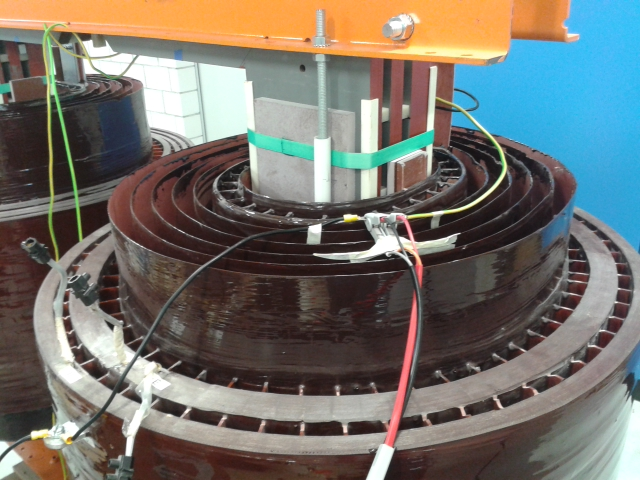
\includegraphics[width=0.5\textwidth]{./trafo/images/resibloc.jpg}
	\caption{Resibloc-Testtransformator der Firma ABB. Zwischen den Layern ist der Luftspalt zur K"uhlung ersichtlich.}
	\label{trafo:resibloc}
\end{figure}
Fr"uher wurde ein Transformator oder allgemein ein elektronisches Betriebsmittel nach Erfahrungen gebaut. Dabei war es gang und g"abe, dass mehrere Prototypen notwendig waren, bis die ersten Spannungspr"ufungen bestanden werden konnten. Deshalb sind CAD-Simulationen wesentlich schneller und vor allem kosteng"unstiger. Das Ziel soll es sein, den Transformator m"oglichst genau darzustellen und dessen Spannungsverteilung zu berechnen, denn die Spannung und die Geometrie zusammen ergeben das elektrische Feld, welches schlussendlich zu Durchschl"agen oder Teilentladungen f"uhrt.

An der Hochschule f"ur Technik Rapperswil wurde am Institut f"ur Energietechnik eine Methode entwickelt, wie die Spannungsverteilung bei einem Blitzstoss m"oglichst genau simuliert werden kann \cite{trafo:BILImpulse}. Diese Methode funktioniert sehr gut f"ur Leistungstransformatoren und konnte mit Messungen auch verifiziert werden. 
Soll dieses Prinzip aber auf Instrumententransformatoren angewendet werden, ergibt die wesentlich h"ohere Anzahl von Windungen und deren engeren Lagen nummerische Probleme mit dem momentanen L"osungsverfahren. 

Diese Probleme werden in diesem Abschnitt schrittweise behandelt und bestm"oglichst gel"ost. 


\subsection{Ersatzschaltbild}
Ein Transformator, ob "ol- oder luftgek"uhlt, kann prinzipiell mit dem Ersatzschaltbild \ref{trafo:einfaches_ESB} dargestellt werden. Dies macht Sinn, wenn der Transformator als Ganzes dargestellt werden will. Soll hingegen die Spannung an jeder Windung berechnet werden, kann dieses bereits bekannte, jedoch zu simple Ersatzschaltbild nicht verwendet werden. Es gilt nun, ein neues und genaueres Ersatzschaltbild zu finden. 

\begin{figure}
	\centering
	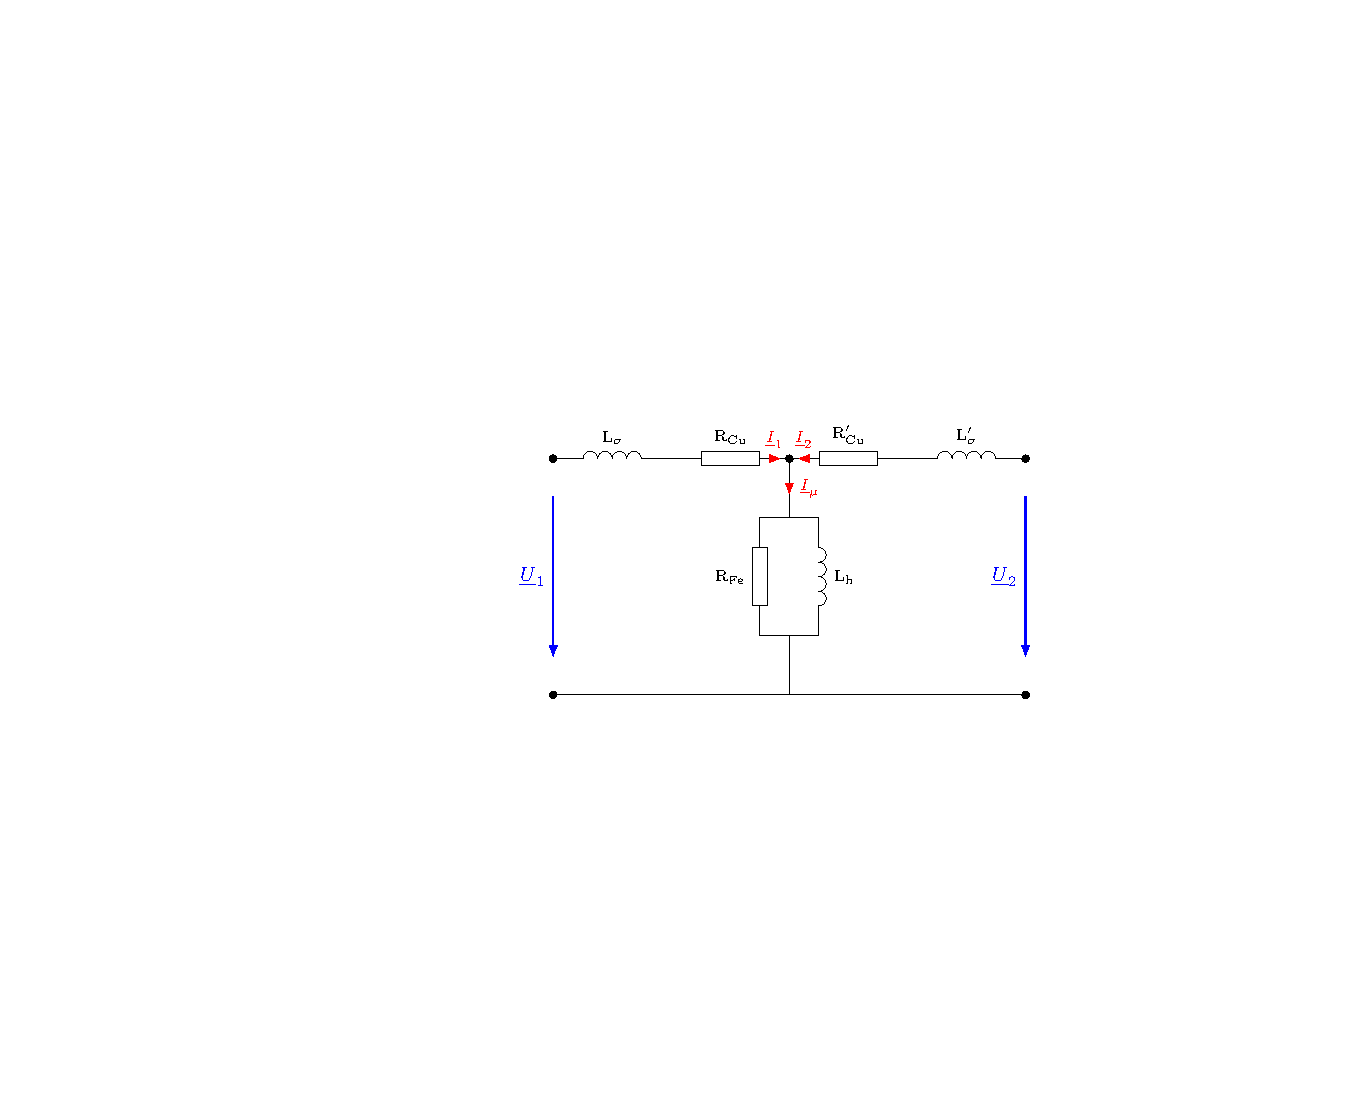
\includegraphics[width=0.7\textwidth]{./trafo/images/Einfaches_ESB.pdf}
	\caption[Einfaches Ersatzschaltbild f"ur einen Transformator]{Einfaches Ersatzschaltbild f"ur einen Transformator.}
	\label{trafo:einfaches_ESB}
\end{figure}

Ein Ansatz ist es, jede Windung einzeln zu modellieren. Pro Windung wird ein elektrischer Widerstand sowie eine Induktivit"at in Serie geschaltet. Ebenfalls m"ussen die Kapazit"aten sowie die Leitf"ahigkeiten gegen"uber Masse und den "ubrigen Windungen ber"ucksichtigt werden \cite{trafo:BILImpulse}. 

Dieses Ersatzschaltbild wird in der Abbildung \ref{trafo:erweitertes_ESB} dargestellt. Als Veranschaulichung wird ein kleines Transformator-Beispiel, bestehend aus 4 Windungen, verwendet. Messungen an Testtransformatoren zeigten, dass ab ca. 20 Windungen die Simulationen mit diesem Ersatzschaltbild sehr genau "ubereinstimmen. 

\begin{figure}
	\centering
	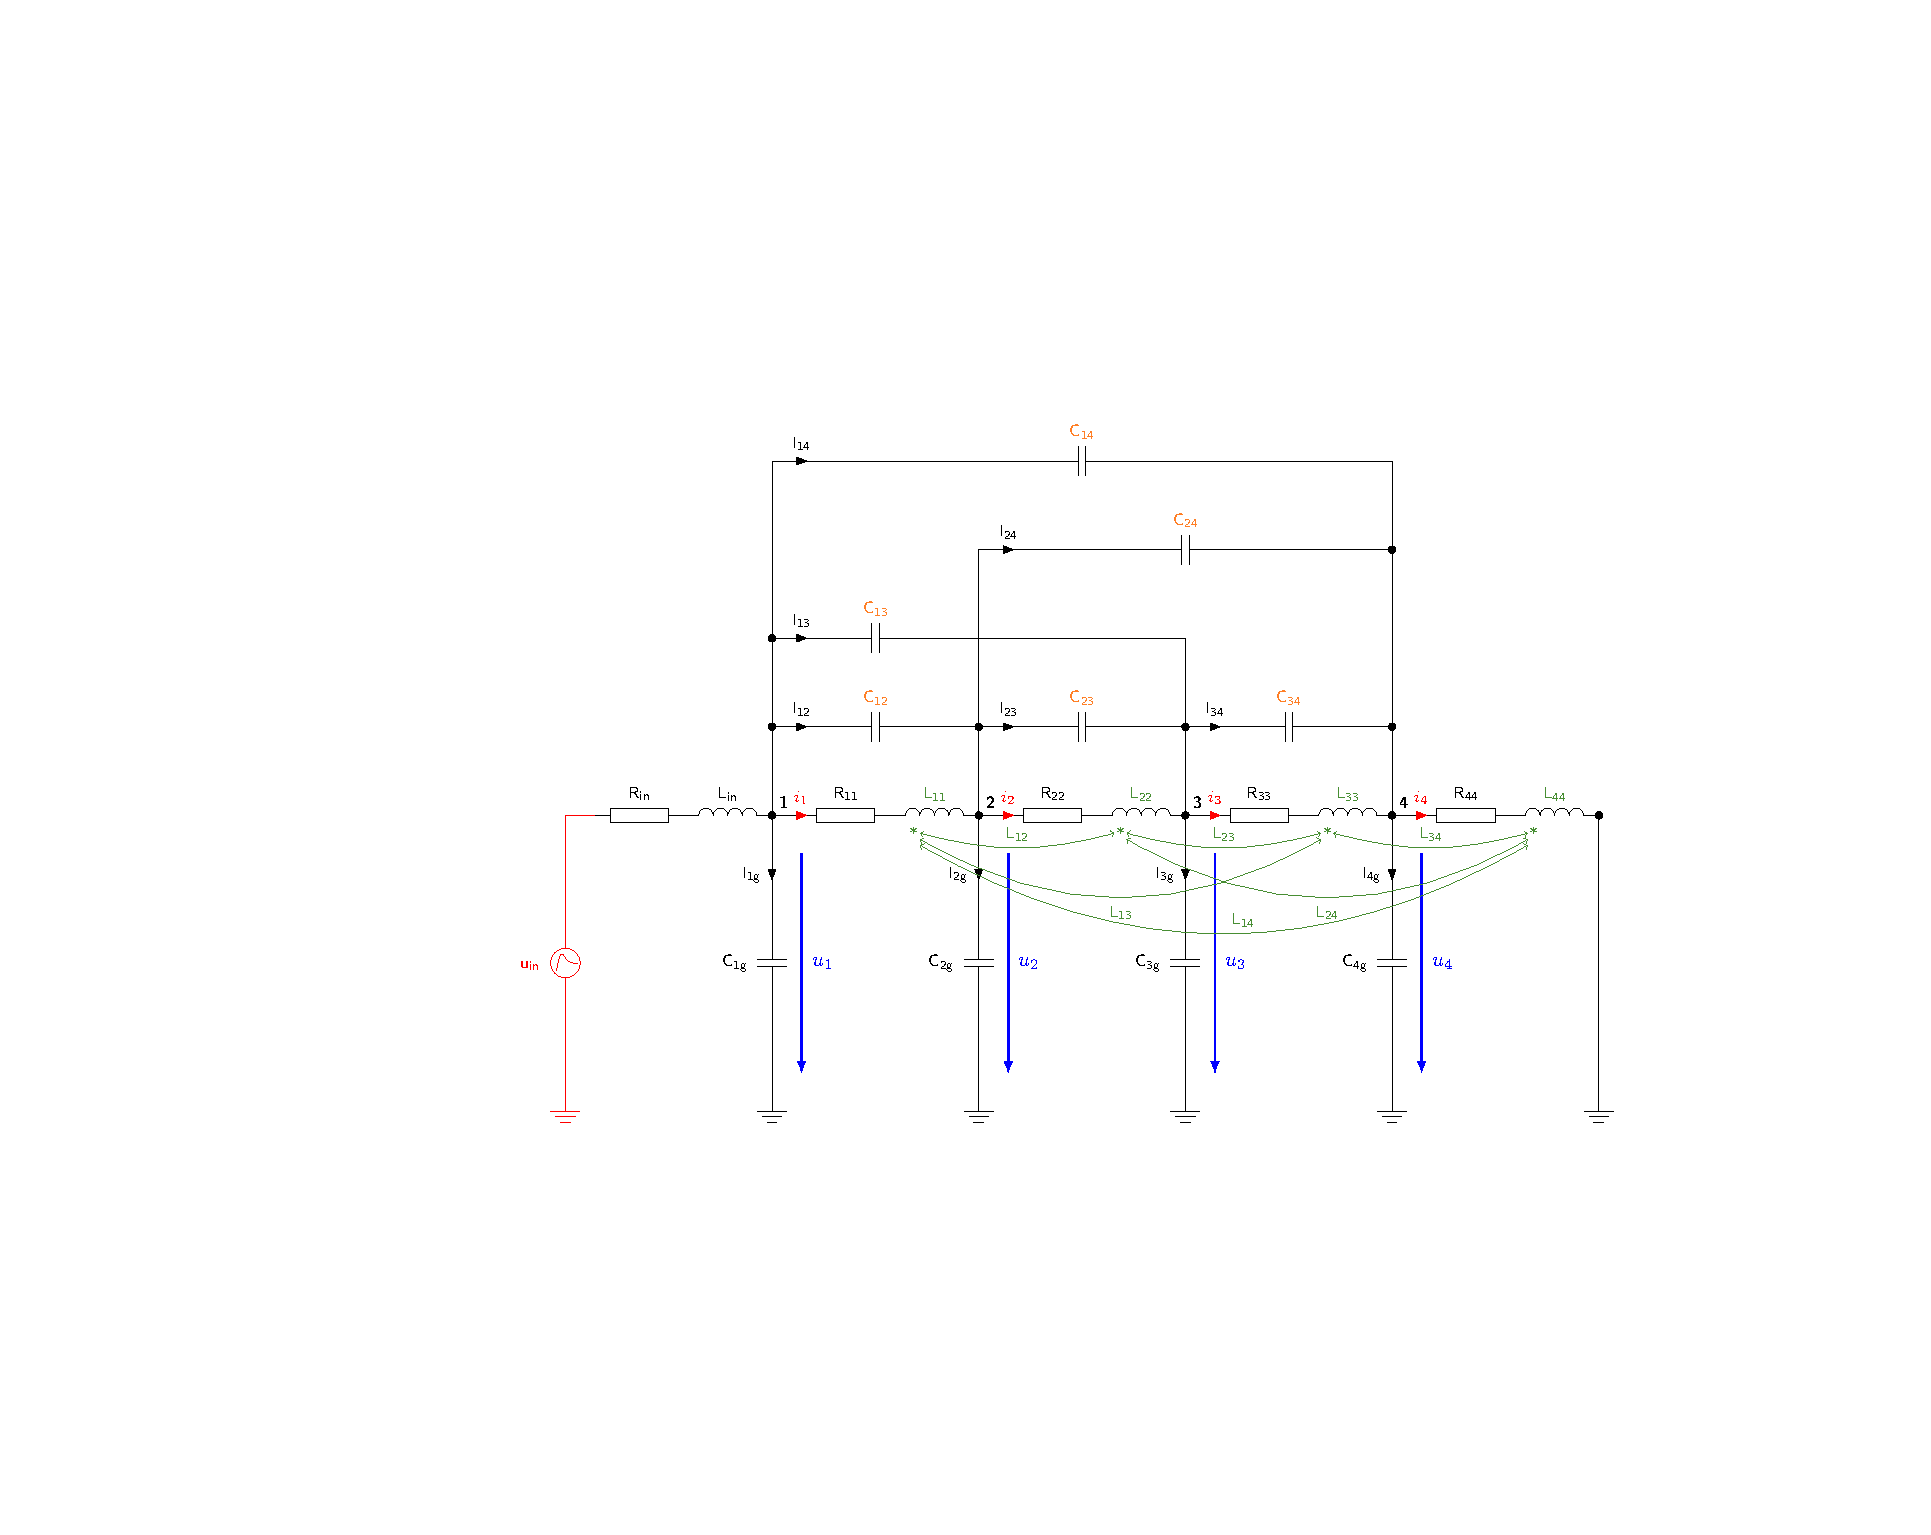
\includegraphics[width=\hsize]{./trafo/images/Trafo_Modell.pdf}
	\caption[Erweitertes Ersatzschaltbild f"ur einen Transformator]{Erweitertes Ersatzschaltbild f"ur einen Transformator mit 4 Windungen. Die Leitwerte zwischen den Windungen und gegen"uber Masse sind auf Grund der "Ubersichtlichkeit weggelassen worden. Die gr"unen Pfeile stellen die Mitkopplung, das heisst die Str"ome welche durch das Eigenfeld einer Windung in die anderen Windungen induziert werden, der Spulen dar. }
	\label{trafo:erweitertes_ESB}
\end{figure}

Damit die Werte der einzelnen Elementen ermittelt werden k"onnen, sind Finite-Element-Methode-(FEM)-Simulationen in einem CAD-Programm notwendig. Das Simulationsmodell im CAD-Programm des Transformators besteht aus in sich geschlossenen Windungen. Weil ein Transformator rotationssymmetrisch ist, kann auf eine rechenintensive 3D Feldsimulation verzichtet und eine (quasi-)2D\footnote{f"ur die Berechnung von elektromagnetische Felder sind immer drei Dimensionen notwendig (man beachte die rechte-Hand-Regel). Wenn das Problem jedoch rotationssymetrisch ist, vereinfachen sich die Felder auf zwei Dimensionen mit einem Stromfluss in der Normale der zweidimensionalen Ebene. Aus diesem Grunde wird diese Simulationsart in CAD-Programmen als '2D' bezeichnet.} Simulation gel"ost werden. Ein Beispiel eines Transformators ist in den Abbildungen \ref{trafo:infolytica} dargestellt.

\begin{figure}
	\centering    
	\subfigure[Ganzer Transformator]{
		\label{fig:a}
		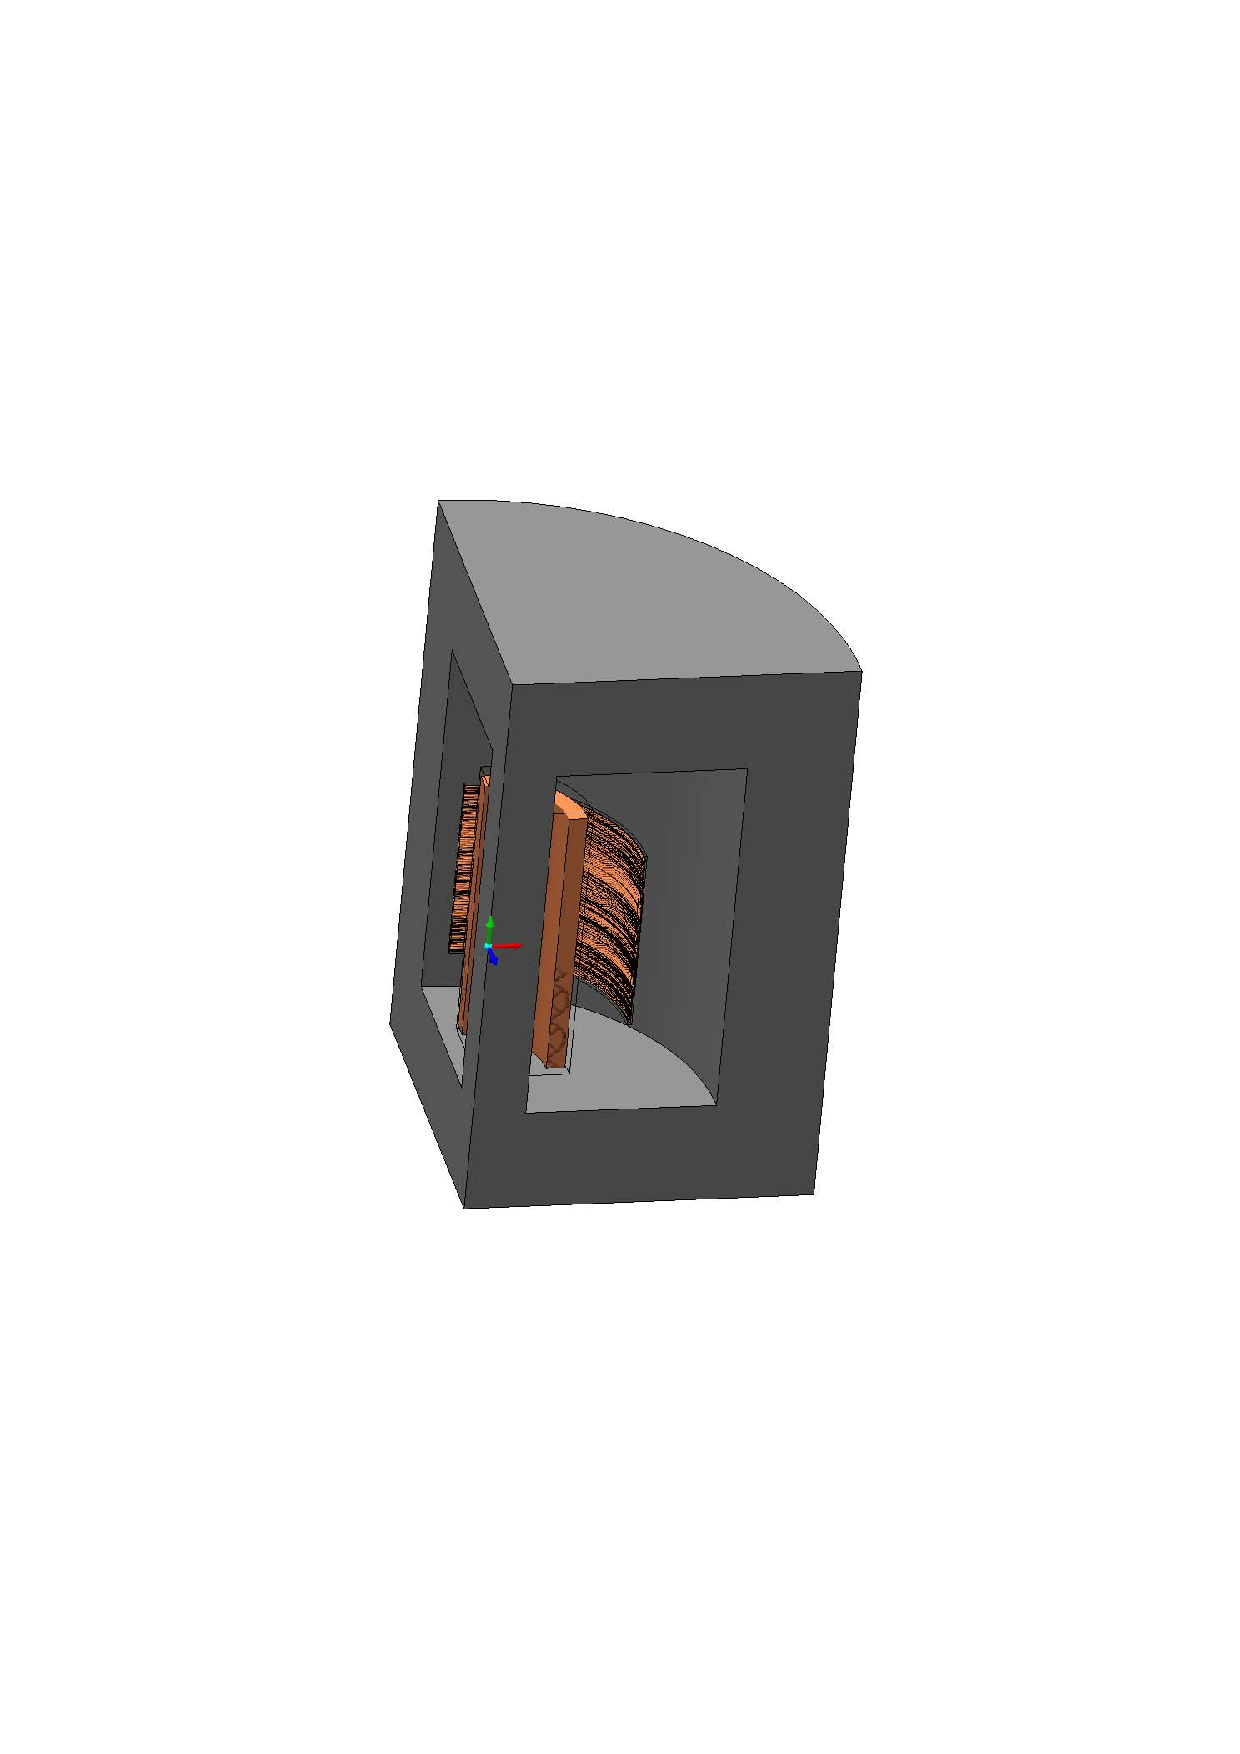
\includegraphics[height=6cm]{./trafo/images/infolytica_ganzer_trafo.pdf}}
	\subfigure[Hochspannungswicklung]{
		\label{fig:b}
		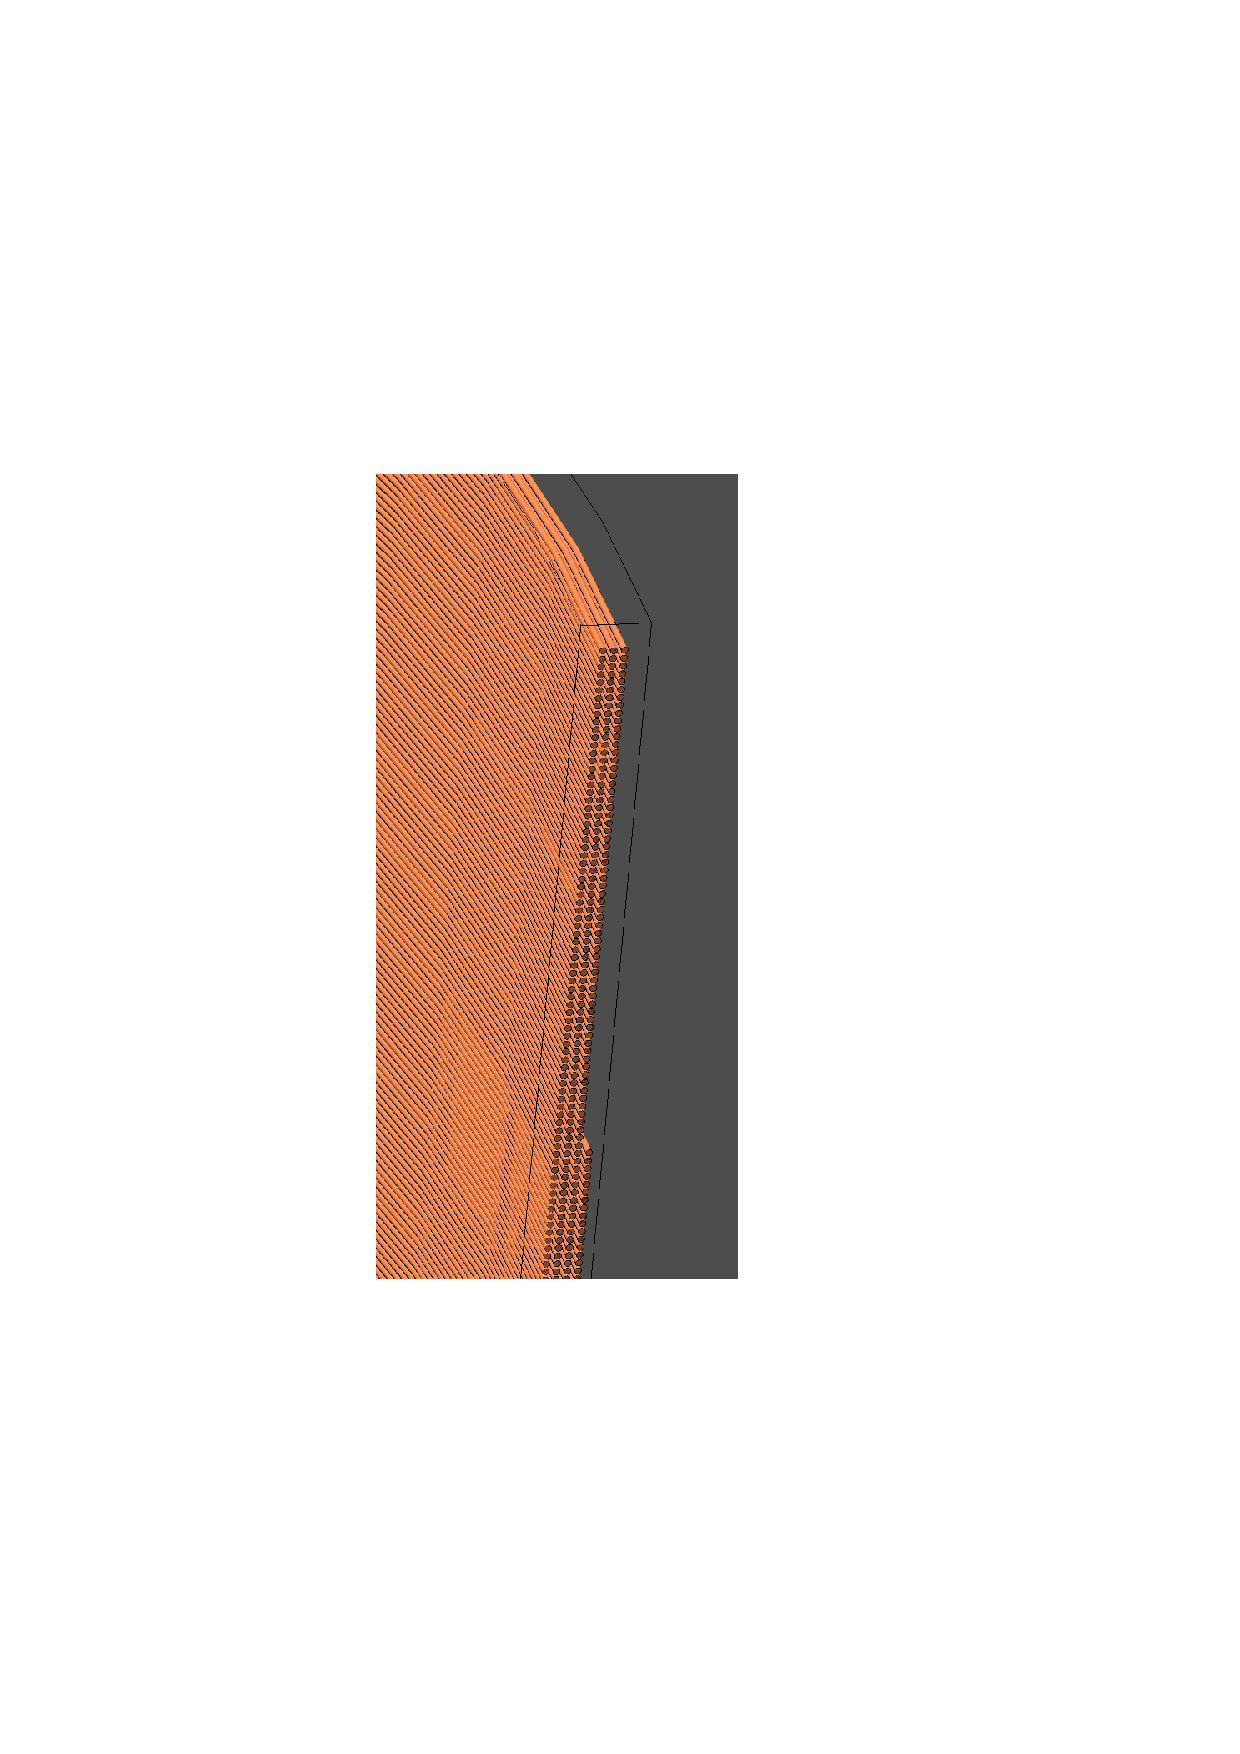
\includegraphics[height=6cm]{./trafo/images/infolytica_windungen.pdf}}
	\caption{Darstellung eines rotationssymmetrischen Transformator in einem CAD-Programm. In \ref{fig:a} ist der ganze Transformator und in \ref{fig:b} ein Ausschnitt der Hochspannungswicklung abgebildet. Jede Windung ist f"ur sich geschlossen moduliert.}
	\label{trafo:infolytica}
\end{figure}

Damit die Ersatzparameter des Transformators mit einer FEM-Simulation berechnet werden k"onnen, wird folgendermassen vorgegangen:
\begin{itemize}
	\item Alle Windungen, abgesehen einer, werden auf das Spannungspotential von  \SI{0}{\volt} gesetzt. 
	\item Diese eine Windung wird an eine Spannungsquelle mit \SI{1}{\volt} angeh"angt.
	\item Es lassen sich nun die Kapazit"aten gegen"uber allen anderen Windungen berechnen.
	\item Das gleiche Vorgehen wird mit der selben Windung an einer Stromquelle verwendet. Die Windung, welche zuvor an der Spannungsquelle angeschlossen war, wird mit \SI{1}{\ampere} Strom durchflossen und alle anderen Windungen mit \SI{0}{\ampere}.
	\item Somit lassen sich die Induktivit"aten berechnen.
	\item Dieser Vorgang wird f"ur jede Windung wiederholt. Somit sind schlussendlich alle Ersatzparameter f"ur das Modell, und ins besonders f"ur das Differentialgleichungssystem \ref{trafo:DGL}, bestimmt.
\end{itemize}


\subsection{Blitzstoss/\textbf{B}asic \textbf{I}nsulation \textbf{L}evel (BIL)}
Als Testspannung wird ein Blitzstoss wie in Abbildung \ref{trafo:BIL} verwendet. Mit diesem Spannungsimpuls soll die Spannungsfestigkeit bei einem Blitzeinschlag gepr"uft werden. Nach Norm muss die Anstiegszeit \SI{1.2}{\micro \second} und die Halbwertsabfallszeit (die Zeit, in welcher die Spannung auf \SI{50}{\percent} absinkt) \SI{50}{\micro \second} betragen. Die H"ohe der Amplitude wird je nach Betriebsspannung in Kategorien eingeteilt, grunds"atzlich betr"agt sie aber ungef"ahr dem 6-fachen der Nennbetriebsspannung. F"ur die Berechnung wird auf Grund der Linearit"at meistens \SI{1}{\volt}, oder auch \textit{pro Einheit} (engl. \textit{per unit} [p.u.]), verwendet. Sp"ater kann dies wieder skaliert werden.

\begin{figure}
	\centering
	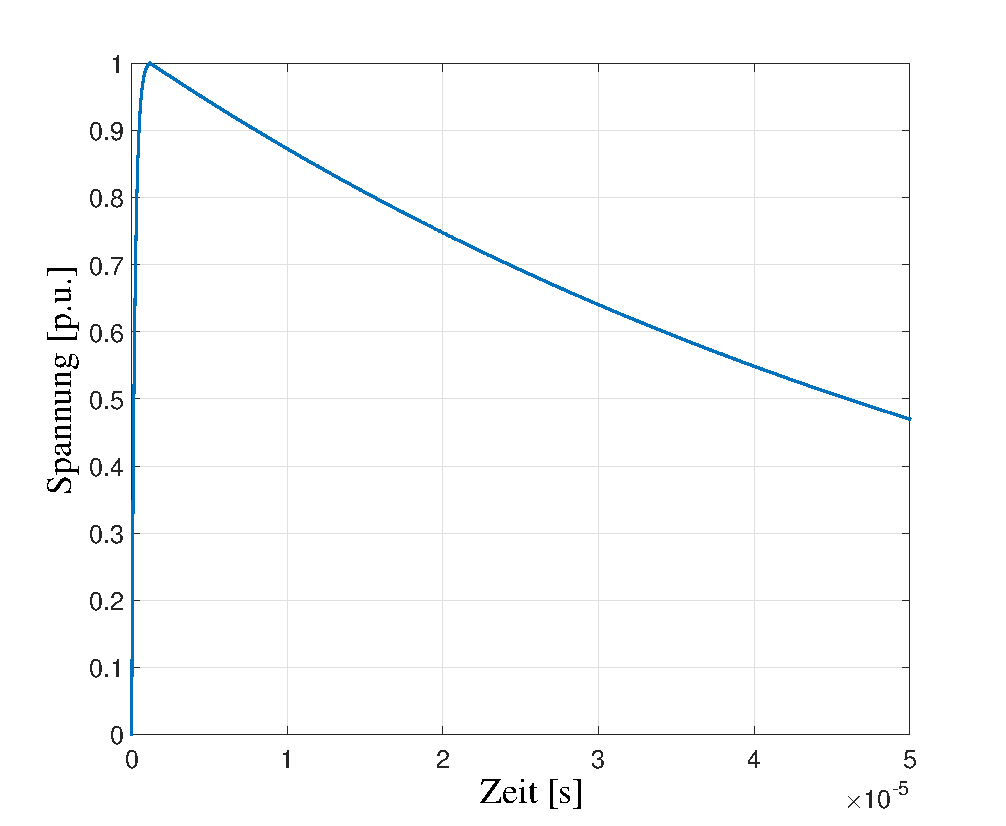
\includegraphics[width=0.6\textwidth]{./trafo/images/pulse.pdf}
	\caption{Normierte Blitzstossspannung zur Testung der Durchschlagsfestigkeit.}
	\label{trafo:BIL}
\end{figure}

\section{Mathematische L"osung}
\subsection{Differentialgleichung}

Nun gilt es, eine Differentialgleichung f"ur das gefundene Ersatzschaltbild aufzustellen. Mittels dem Maschensatz (blaue Pfeile) und der Knotenpunktregel (rote Punkte) k"onnen die Differentialgleichungen pro Windung aufgestellt werden (dargestellt Abbildung in \ref{trafo:orig}).

\begin{figure}
	\centering
	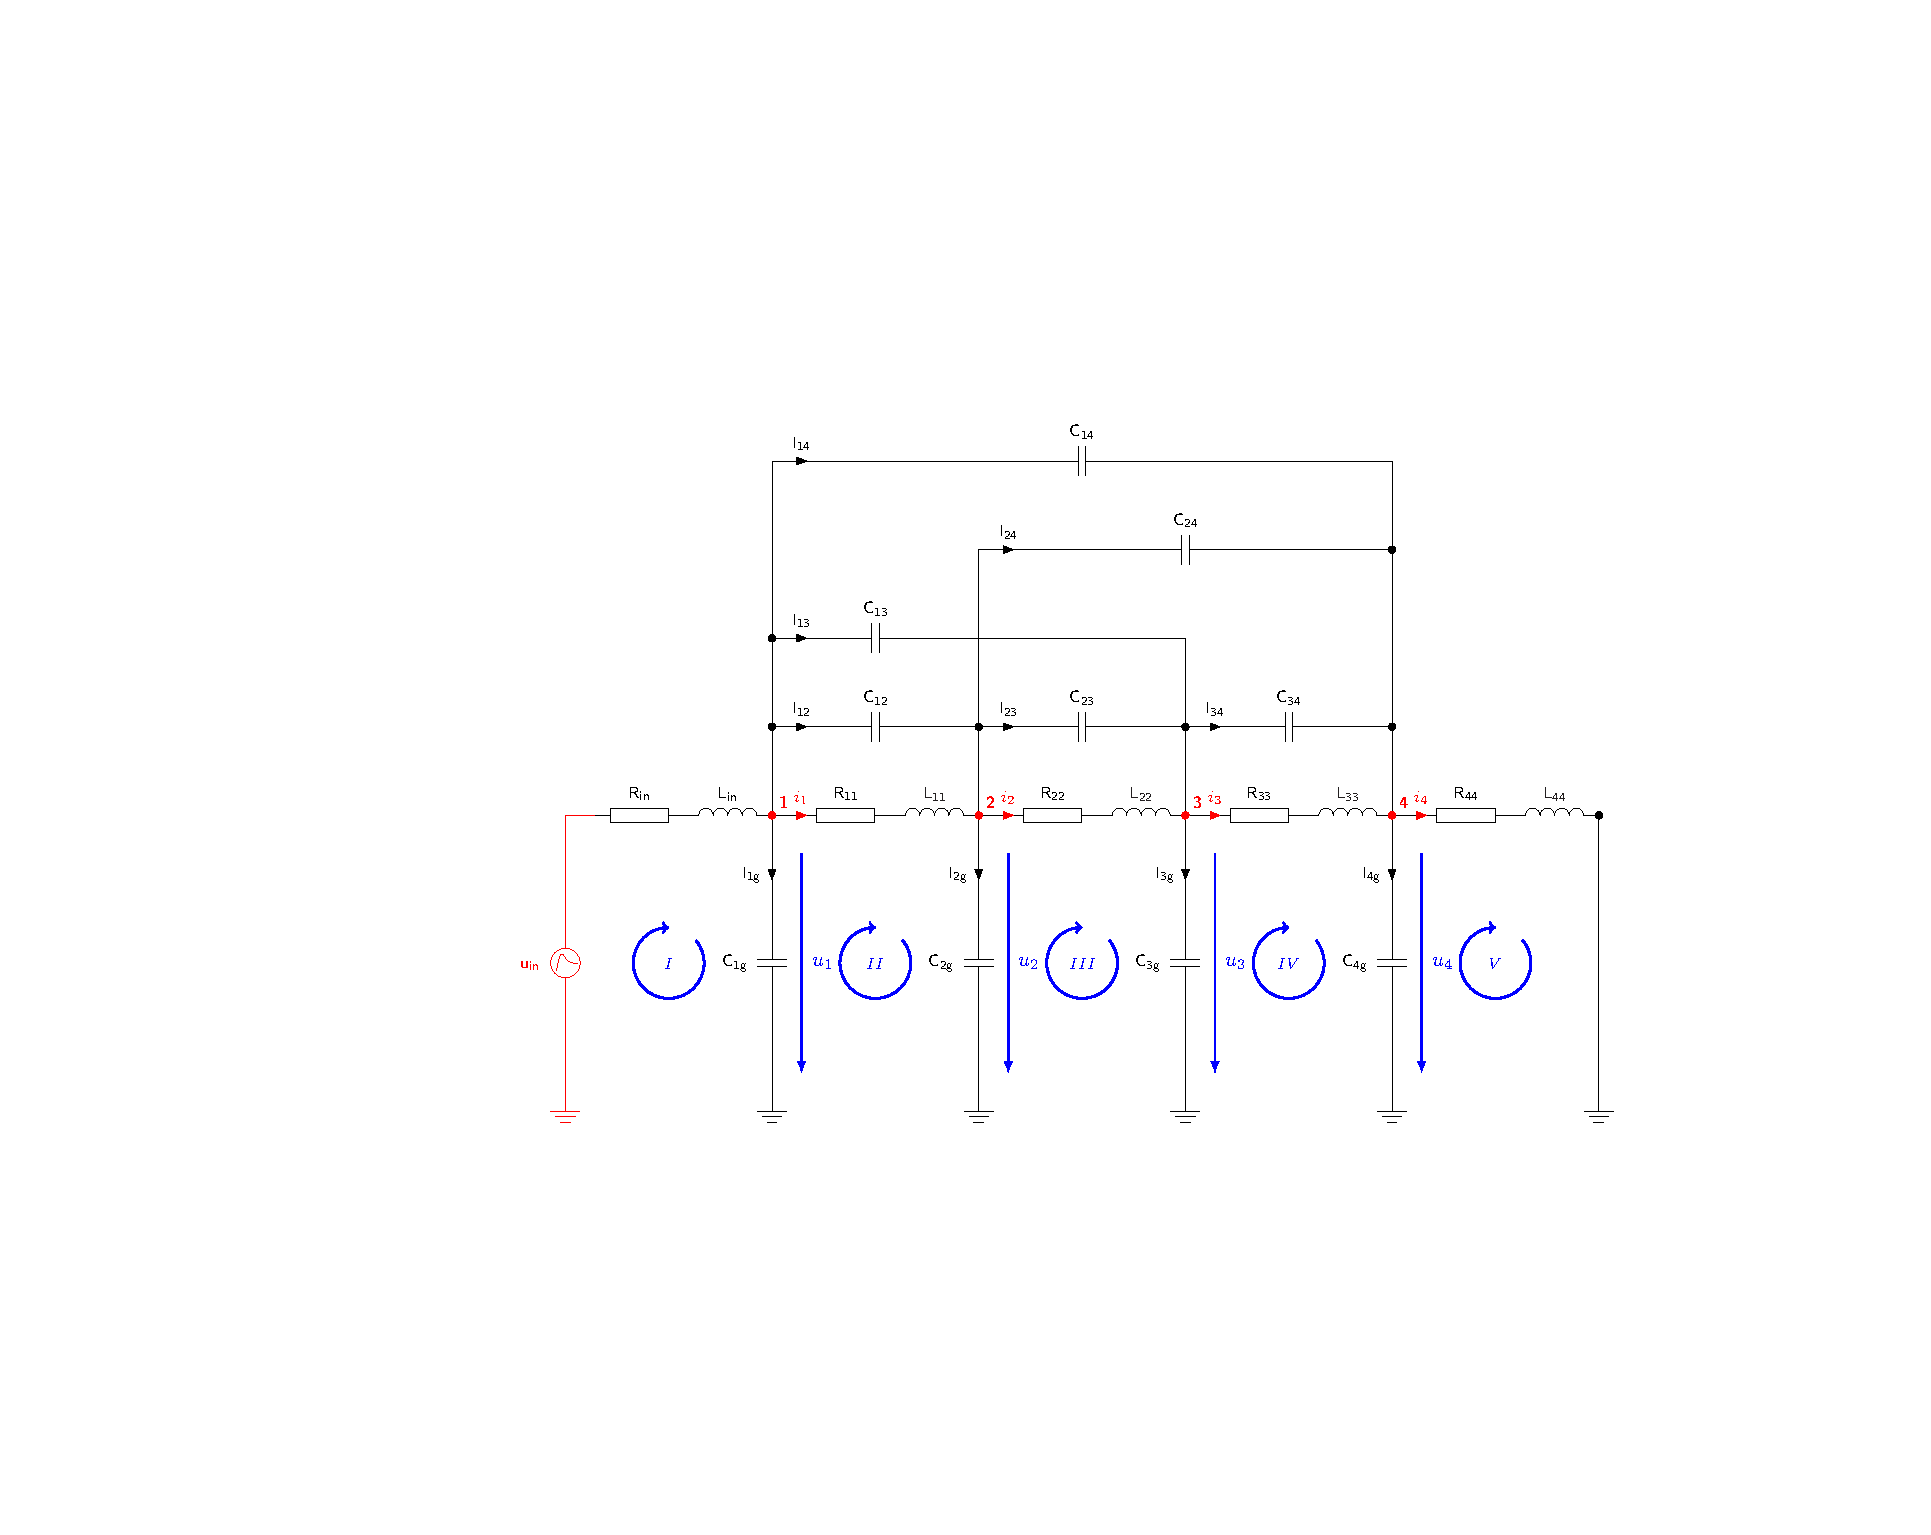
\includegraphics[width=\hsize]{./trafo/images/orig_trafo.pdf}
	\caption[Erweitertes Ersatzschaltbild f"ur einen Transformator mit Maschensatz und Knotenpunkt]{Erweitertes Ersatzschaltbild f"ur einen Transformator mit 4 Windungen. Die blauen Pfeil stellen den Maschensatz und die roten Punkte die Knotenpunktregel dar.}
	\label{trafo:orig}
\end{figure}

Beispielsweise kann die Gleichungen der Windung 1 als 

\begin{equation}
	u_\mathrm{Rin} + u_\mathrm{Lin} + u_1 = u_\mathrm{in}
\end{equation}
und 
\begin{equation}
	i_\mathrm{in} = i_1 + i_{C1g} + i_{R12} + i_{C12} + i_{R13} + i_{C13} + i_{R14} + i_{C14}
\end{equation}
geschrieben werden. Aus den Zusammenfassungen der Str"ome
\begin{equation*}
	\sum i_{C1k} = i_{C1g}+ i_{C12} + i_{C13} + i_{C14}
\end{equation*}
und
\begin{equation*}
	\sum i_{R1k} = i_{R12} + i_{R13} + i_{R14}
\end{equation*}
resultieren die Ersatzparameter $\sum C_{1k}$ und $\sum R_{1k}$ respektive $\sum G_{1k}$, welche in den Gleichungen \ref{trafo:DGL} und \ref{trafo:symmetricalDGL} verwendet werden.

Mit einigen Umformungen kann der ganze Transformator als System mehreren Differentialgleichungen geschrieben werden \cite{trafo:SeminarCHR}. Als Beispiel wird wiederum der Transformator mit 4 Windungen gew"ahlt. Der Vektor $E$ ist der St"orterm des Systems, welcher in diesem Falle der Blitzstoss ist.

{\footnotesize 
\begin{align}
			&
			\underbrace{\begin{bmatrix}
			L_\mathrm{in}&0&0&0&0 & 0&0&0&0 \\
			0&L_{11}&L_{12}&L_{13}&L_{14} & 0&0&0&0 \\
			0&L_{21}&L_{22}&L_{23}&L_{24} & 0&0&0&0 \\
			0&L_{31}&L_{32}&L_{33}&L_{34} & 0&0&0&0 \\
			0&L_{41}&L_{42}&L_{43}&L_{44} & 0&0&0&0 \\
			0&0&0&0&0 & \sum{C_{1k}}&-C_{12}&-C_{13}&-C_{14} \\
			0&0&0&0&0 & -C_{21}&\sum{C_{2k}}&-C_{23}&-C_{24} \\
			0&0&0&0&0 & -C_{31}&-C_{32}&\sum{C_{3k}}&-C_{34} \\
			0&0&0&0&0 & -C_{41}&-C_{42}&-C_{43}&\sum{C_{4k}}
			    \end{bmatrix}}_{\text{$M$}}
			\cdot
			\underbrace{\begin{bmatrix}
			\frac{di_\mathrm{in}}{dt} \\
			\frac{di_1}{dt} \\
			\frac{di_2}{dt} \\
			\frac{di_3}{dt} \\
			\frac{di_4}{dt} \\
			\frac{du_1}{dt} \\
			\frac{du_2}{dt} \\
			\frac{du_3}{dt} \\
			\frac{du_4}{dt}
			\end{bmatrix}}_{\text{$\dot{x}$}}
			= \nonumber \\
			&
			\underbrace{\begin{bmatrix}
			-R_\mathrm{in}&0&0&0&0 & -1&0&0&0 \\
			0&-R_{11}&0&0&0 & 1&-1&0&0 \\
			0&0&-R_{22}&0&0 & 0&1&-1&0 \\
			0&0&0&-R_{33}&0 & 0&0&1&-1 \\
			0&0&0&0&-R_{44} & 0&0&0&1 \\
			1&-1&0&0&0 & -\sum G_{1k}&G_{12}&G_{13}&G_{14} \\
			0&1&-1&0&0 & G_{21} &- \sum G_{2k}& G_{23}& G_{24} \\
			0&0&1&-1&0 & G_{31} & G_{32} &-\sum G_{3k}&G_{34} \\
			0&0&0&1&-1 & G_{41}&G_{42}&G_{43}&-\sum G_{4k}
			\end{bmatrix}}_{\text{$N$}}
			\cdot
			\underbrace{\begin{bmatrix}
			i_\mathrm{in} \\
			i_1 \\
			i_2 \\
			i_3 \\
			i_4 \\
			u_1 \\
			u_2 \\
			u_3 \\
			u_4
			\end{bmatrix}}_{\text{$x$}}
			+
			\underbrace{\begin{bmatrix}
			u_\mathrm{in} \\
			0 \\
			0 \\
			0 \\
			0 \\
			0 \\
			0 \\
			0 \\
			0
			\end{bmatrix}}_{\text{$E$}}
			\label{trafo:DGL}
\end{align}
}
		


Die Matrix $M$ ist eine symmetrische Matrix, was f"ur weitere Berechnungen wesentliche Vorteile mit sich bringt. Die Matrix $N$ ist fast symmetrisch. Wenn der Maschensatz jedoch in die andere Richtung als in Abbildung \ref{trafo:orig} angewendet wird, l"asst sich auch diese Matrix mit sehr geringem Aufwand in die symmetrische Form bringen. Dies ist f"ur dieses Beispiel zwar nicht n"otig, trotzdem kann es f"ur andere L"osungsans"atze von Vorteil sein. Aus der Gleichung \ref{trafo:DGL} wird nun 

{\footnotesize 
\begin{align}
			&
			\underbrace{\begin{bmatrix}
			\color{red}-\color{black}L_\mathrm{in}&0&0&0&0 & 0&0&0&0 \\
			0&\color{red}-\color{black}L_{11}&\color{red}-\color{black}L_{12}&\color{red}-\color{black}L_{13}&\color{red}-\color{black}L_{14} & 0&0&0&0 \\
			0&\color{red}-\color{black}L_{21}&\color{red}-\color{black}L_{22}&\color{red}-\color{black}L_{23}&\color{red}-\color{black}L_{24} & 0&0&0&0 \\
			0&\color{red}-\color{black}L_{31}&\color{red}-\color{black}L_{32}&\color{red}-\color{black}L_{33}&\color{red}-\color{black}L_{34} & 0&0&0&0 \\
			0&\color{red}-\color{black}L_{41}&\color{red}-\color{black}L_{42}&\color{red}-\color{black}L_{43}&\color{red}-\color{black}L_{44} & 0&0&0&0 \\
			0&0&0&0&0 & \sum{C_{1k}}&-C_{12}&-C_{13}&-C_{14} \\
			0&0&0&0&0 & -C_{21}&\sum{C_{2k}}&-C_{23}&-C_{24} \\
			0&0&0&0&0 & -C_{31}&-C_{32}&\sum{C_{3k}}&-C_{34} \\
			0&0&0&0&0 & -C_{41}&-C_{42}&-C_{43}&\sum{C_{4k}}
			    \end{bmatrix}}_{\text{$M$}}
			\cdot
			\underbrace{\begin{bmatrix}
			\frac{di_\mathrm{in}}{dt} \\
			\frac{di_1}{dt} \\
			\frac{di_2}{dt} \\
			\frac{di_3}{dt} \\
			\frac{di_4}{dt} \\
			\frac{du_1}{dt} \\
			\frac{du_2}{dt} \\
			\frac{du_3}{dt} \\
			\frac{du_4}{dt}
			\end{bmatrix}}_{\text{$\dot{x}$}}
			= \nonumber \\
			&
			\underbrace{\begin{bmatrix}
			\color{red}+\color{black}R_\mathrm{in}&0&0&0&0 & \color{red}+\color{black}1&0&0&0 \\
			0&\color{red}+\color{black}R_{11}&0&0&0 & \color{red}-\color{black}1&\color{red}+\color{black}1&0&0 \\
			0&0&\color{red}+\color{black}R_{22}&0&0 & 0&\color{red}-\color{black}1&\color{red}+\color{black}1&0 \\
			0&0&0&\color{red}+\color{black}R_{33}&0 & 0&0&\color{red}-\color{black}1&\color{red}+\color{black}1 \\
			0&0&0&0&\color{red}+\color{black}R_{44} & 0&0&0&\color{red}-\color{black}1 \\
			1&-1&0&0&0 & -\sum G_{1k}&G_{12}&G_{13}&G_{14} \\
			0&1&-1&0&0 & G_{21} &- \sum G_{2k}& G_{23}& G_{24} \\
			0&0&1&-1&0 & G_{31} & G_{32} &-\sum G_{3k}&G_{34} \\
			0&0&0&1&-1 & G_{41}&G_{42}&G_{43}&-\sum G_{4k}
			\end{bmatrix}}_{\text{$N$}}
			\cdot
			\underbrace{\begin{bmatrix}
			i_\mathrm{in} \\
			i_1 \\
			i_2 \\
			i_3 \\
			i_4 \\
			u_1 \\
			u_2 \\
			u_3 \\
			u_4
			\end{bmatrix}}_{\text{$x$}}
			\color{red}-\color{black}
			\underbrace{\begin{bmatrix}
			u_\mathrm{in} \\
			0 \\
			0 \\
			0 \\
			0 \\
			0 \\
			0 \\
			0 \\
			0
			\end{bmatrix}}_{\text{$E$}}
			\label{trafo:symmetricalDGL}
\end{align}
}

Dieses System mehrerer Differentialgleichungen kann auch mit Matrizen und Vektoren geschrieben werden, welches sich etwas "ubersichtlicher darstellen l"asst. 

\begin{equation}
	M \dot x = N x + E
	\label{trafo:matricesDGL}
\end{equation}

Wird die Massenmatrix $M$ auf die rechte Seite der Gleichung \ref{trafo:matricesDGL} dividiert, ergibt dies

\begin{equation}
	\dot{x} = M^{-1}N x + M^{-1} E = A x + B
\end{equation}
welches die allgemein bekannte und auch l"osbare Zustandsraumdarstellung \index{Zustandsraumdarstellung} (engl. state space) ist.

Das Problem scheint bereits gel"ost zu sein, wenn sich die Massenmatrix $M$ invertieren l"asst. In der Theorie w"are dies tats"achlich auch machbar, jedoch sehr aufw"andig. Weil auch gewisse Eigenwerte zu klein sind, explodiert die L"osung und kann somit mit diesem Ansatz nicht gel"ost werden.

Folglich muss ein Ansatz gefunden werden, welcher die Massenmatrix $M$ m"oglichst ressourcenschonend invertiert und eine numerisch konvergierende L"osung ergibt. 


\subsection{Singular Value Decomposition (SVD) \index{Singular Value Decomposition}}
Eine M"oglichkeit stellt die Singular Value Decomposition, zu Deutsch Singul"arwertzerlegung, dar. Ohne Gedanken "uber die Dimensionen der Matrix $M$ zu verlieren, wird der SVD-Satz verwendet \cite{trafo:Watkins}. 

\begin{satz}
	\label{trafo:SVDTheorem}
	(\textit{SVD Theorem}) Sei $M\in \mathbb{R}^{n \times m}$ eine besetzte Matrix mit Rang $r$. Dann kann $M$ als Produkt
	\begin{equation}
		M = USV^\top
		\label{trafo:svd}
	\end{equation} 
	geschrieben werden, wobei $U \in \mathbb{R}^{n \times n}$ und $V \in \mathbb{R}^{m \times m}$ orthogonal sind und $S \in \mathbb{R}^{n \times m}$ eine rechteckige Diagonalmatrix ist 
	\begin{equation*}
		S = \left( 
			\begin{array}{ccc|ccc}
				\sigma_1 &          &          &        & \vdots &        \\
				& \ddots   &          & \cdots & 0      & \cdots \\
				&          & \sigma_r &        & \vdots &        \\
				\hline
				&  \vdots  &          &        & \vdots &        \\
				\cdots   &  0       & \cdots   & \cdots & 0      & \cdots \\
				&  \vdots  &          &        & \vdots &   \\				
				\end{array}
			\right) 
			\hspace{2cm}\sigma_1 \geq \sigma_2 \geq \dots \sigma_r > 0. 
	\end{equation*}
\end{satz}
F"ur die Herleitung und den Beweis des Satzes \ref{trafo:SVDTheorem} wird auf die Fachliteratur verwiesen \cite{trafo:Watkins}.

Einfach erkl"aren l"asst sich die Singul"arwertzerlegung mit jeweils zwei Rotationen, es sind dies die Matrizen $U$ und $V^\top$, und einer Streckung durch die Diagonalmatrix $S$. Dieser Vorgang ist in Abbildung \ref{trafo:SVDFig} dargestellt. 

Eine einfache Art die Singul"arwertzerlegung von $M$ zu bekommen, ist die Berechnung der Eigenwerten und Eigenvektoren von $M^\top M \in \mathbb{R}^{m \times m}$ und $MM^\top \in \mathbb{R}^{n \times n}$. Die Matrix $U$ ist aus Eigenvektoren von $MM^\top$ aufgebaut welche mit
\begin{equation*}
	\left(\lambda_i E - MM^\top\right)u_i = 0
\end{equation*}
berechnet werden können, wobei $\lambda_i$ die Eigenwerte von $MM^\top$ sind und $E$ die Einheitsmatrix ist. Die Matrix $U$ besitzt somit in der Senkrechte Eigenvektoren \cite{trafo:Watkins}.
\begin{equation*}
	\left( 
		\begin{array}{cccc}
		u_1 & u_2 & \dots & u_n  \\		
		\end{array}
	\right)
\end{equation*}

Die Matrix $V$ kann mit dem selben Schema aus den Eigenvektoren von $M^\top M$ aufgebaut werden. Als etwas schnellere Alternative kann die Berechnung von $V$ jedoch auch aus der Gleichung \ref{trafo:svd} erfolgen, denn $M$, $S$ und $U$ sind bekannt. 
\begin{align*}
	M^\top &= V \underbrace{S^\top}_{S} U^\top\\
	S^{-1} M^\top &= V U^\top\\
	V &= S^{-1} M^\top \left(U^\top\right) = S^{-1} M^\top U
\end{align*}
Die Matrix $V$ besitzt in der Vertikale Eigenvektoren  \cite{trafo:Watkins}
\begin{equation*}
	\left( 
		\begin{array}{c}
		{v_1}^{\top}\\
		{v_2}^{\top}\\
		\vdots\\
		{v_m}^{\top}\\			
		\end{array}
	\right).
\end{equation*}

\begin{figure}
	\centering
	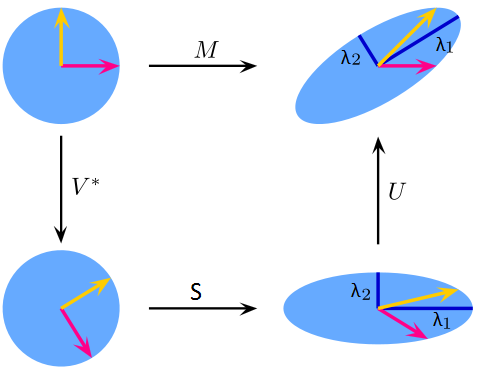
\includegraphics[width=0.4\textwidth]{./trafo/images/svd.png}
	\caption{Grafische Darstellung der Singul"arwertzerlegung \cite{trafo:SVDWiki}.}
	\label{trafo:SVDFig}
\end{figure}

Da es sich bei der Matrix $M$ um eine symmetrische Matrix handelt, sind die Singul"arwerte $\sigma$ in der Matrix $S$ sogleich die Eigenwerte $\lambda$ der Matrix $M$.

\subsubsection{Unterdr"uckung von unerw"unschten Eigenwerten}
Die rechteckige Diagonalmatrix $S$ wird wegen der symmetrischen Matrix $M$ zu einer quadratischen Matrix. Dies bedeutet, dass sich auf der ganzen Diagonale Betr"age von Eigenwerten des Systems befinden. Ein Ansatz zur Unterdr"uckung unerw"unschten Frequenzen kann sein, zu kleine Eigenwertbetr"age $\lambda < \text{tol}$, welche numerischen L"osungsverfahren nicht folgen k"onnen und physikalisch gesehen zu grosse und unm"ogliche Frequenzen sind, auf Null zu setzen. Dies ergibt die Diagonalmatrix 
\begin{equation*}
	S_\text{tol} = \left( 
			\begin{array}{cccccc}
				\lambda_1 & & & & & \\
				& \ddots & & & &  \\
				& & \lambda_{\text{tol}} & & & \\
				& & & 0 & & \\
				& & & & \ddots & \\
				& & & & & 0 \\				
				\end{array}
			\right) 
			\hspace{2cm}\lambda_1 \geq \lambda_2 \geq \dots \lambda_{\text{tol}} > 0. 
\end{equation*}
Die Matrix $S_\text{tol}$ ist eine reduzierte Matrix, welche nur die Singulärwerte bis zum Toleranzwert beinhaltet, die kleineren Werte werden durch $0$ ersetzt. Diese Matrix lässt sich noch nicht invertieren, da bekanntlich nicht durch $0$ geteilt werden darf. Die Pseudoinverse $S{_\text{tol}}^\dagger$ löst dieses Problem, indem sie die vorhandene Werte invertiert und die Nullen stehen lässt.\footnote{Matlab bietet bereit eine Funktion \texttt{pinv(M,tol)} an, welche jedoch langsamer wie die Implementation in \ref{trafo:SVD} ist und deshalb nicht verwendet wird.} Somit ist $S{_\text{tol}}^\dagger$ die Pseudoinverse der reduzierten Singulär-Matrix.

\subsubsection{Inversion}
Als n"achstes gilt es, eine einfache 'Inversion' der Matrix $M$ zu finden. Bis anhin wurde die Singul"arwertzerlegung angewendet, in der Annahme, schlussendlich eine Vereinfachung der Inversion zu finden. Die Inversion zeigt tats"achlich, dass sich einiges vereinfachen l"asst. \cite{trafo:Watkins}
\begin{equation*}
	M^{-1} = \left(U S{_\text{tol}}^\dagger V^\top\right)^{-1} = \left(V^\top\right)^{-1} \left(S{_\text{tol}}^\dagger\right)^{-1} U^{-1}
\end{equation*}
Da die Matrizen $U$ und $V$ symmetrisch sind, gilt $U^{-1} = U^\top$ und $\left(V^\top\right)^{-1} = V$. Dadurch kann die Gleichung als 
\begin{equation*}
	M^{-1} = V \left(S{_\text{tol}}^\dagger \right)^{-1} U^\top
\end{equation*}
geschrieben werden.

Dies ist wesentlich schneller zu berechnen als die Inverse der Matrix $M$, da lediglich die Diagonalmatrix invertiert werden muss.

\subsubsection{Implementation \label{trafo:SVD}}
Die Implementation in Matlab l"asst sich sehr kompakt und elegant darstellen. Wie soeben erkl"art werden zu kleine Eigenwerte auf Null gesetzt und anschliessend die Inverse berechnet. 

{\scriptsize \lstinputlisting{./trafo/code/svd.m}}

\subsubsection{Resultate}
Damit der Wert der Toleranz bestimmt werden kann, m"ussen ein paar Testl"osungen erstellt werden. Als L"osungsverfahren wurde das etwas langsame, jedoch genaue nummerische Verfahren \texttt{ode45} von Matlab verwendet. In der Abbildung \ref{trafo:SVDTol} lassen sich die Unterschiede der gew"ahlten Toleranzen sehr gut erkennen. Wenn die Toleranzen $10^{-11}$ und $10^{-12}$ gew"ahlt werden, l"asst sich das Problem l"osen, jedoch ist das Verhalten des Systems erfahrungsgem"ass nicht ganz realistisch. Die L"osung mit der Toleranz $10^{-13}$ zeigt, wie es in der Praxis tats"achlich aussehen sollte. Wird die Toleranz hingegen noch einmal etwas verringert, explodiert die L"osung und ist somit nicht mehr brauchbar. Dieser Fall ist in Abbildung \ref{trafo:SVDTol} unten rechts dargestellt.

	\begin{figure}
	    \centering
	    \begin{minipage}{.5\textwidth}
	        \centering
	        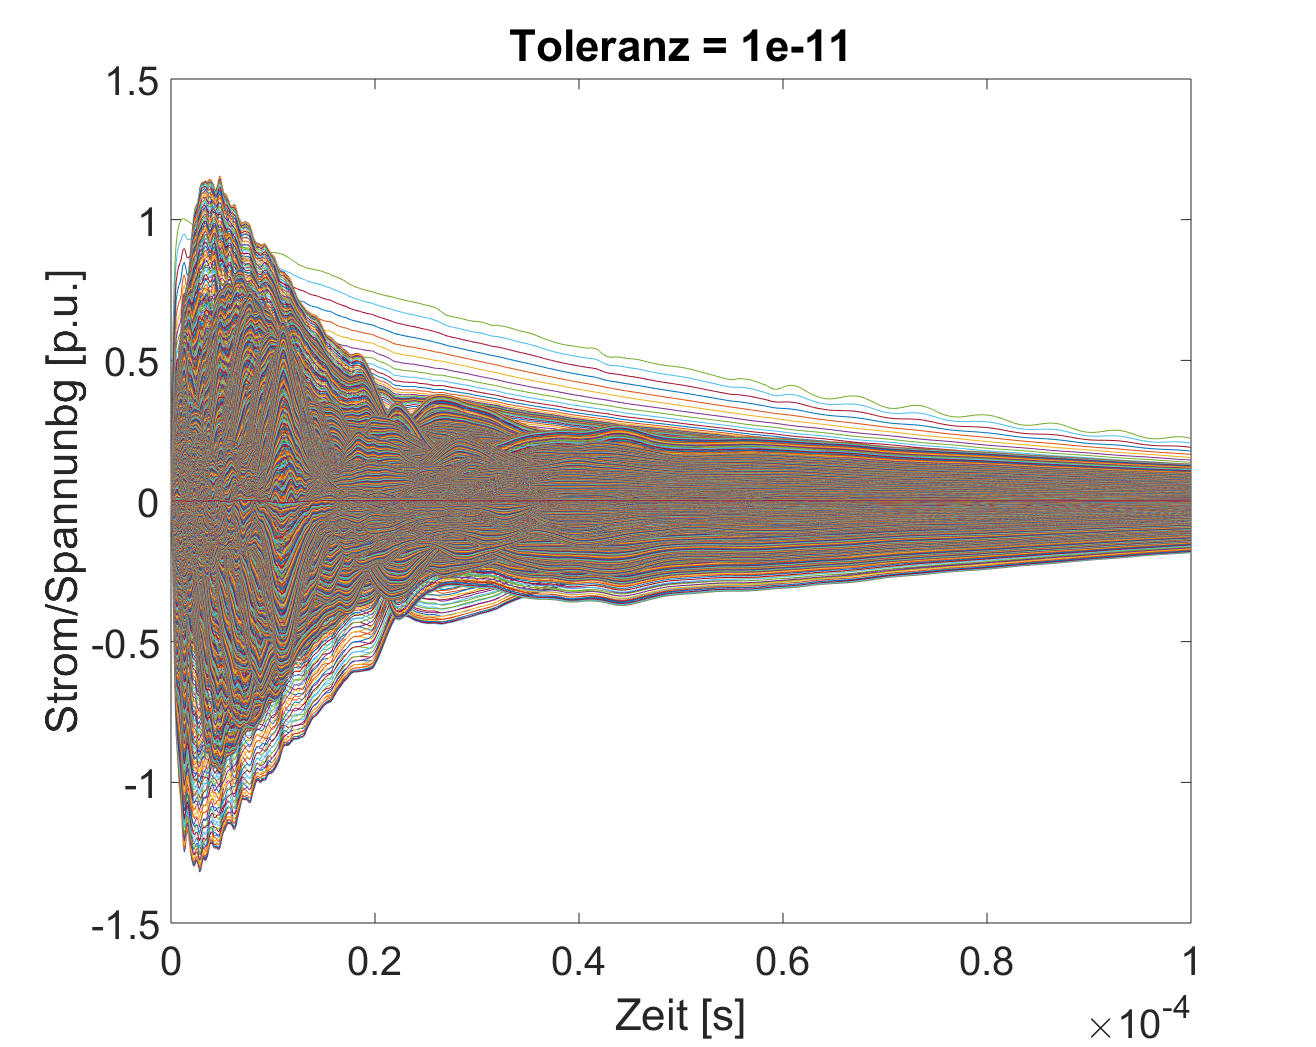
\includegraphics[width=\linewidth]{./trafo/images/svd11.png}
	    \end{minipage}%
	    \begin{minipage}{.5\textwidth}
	        \centering
	        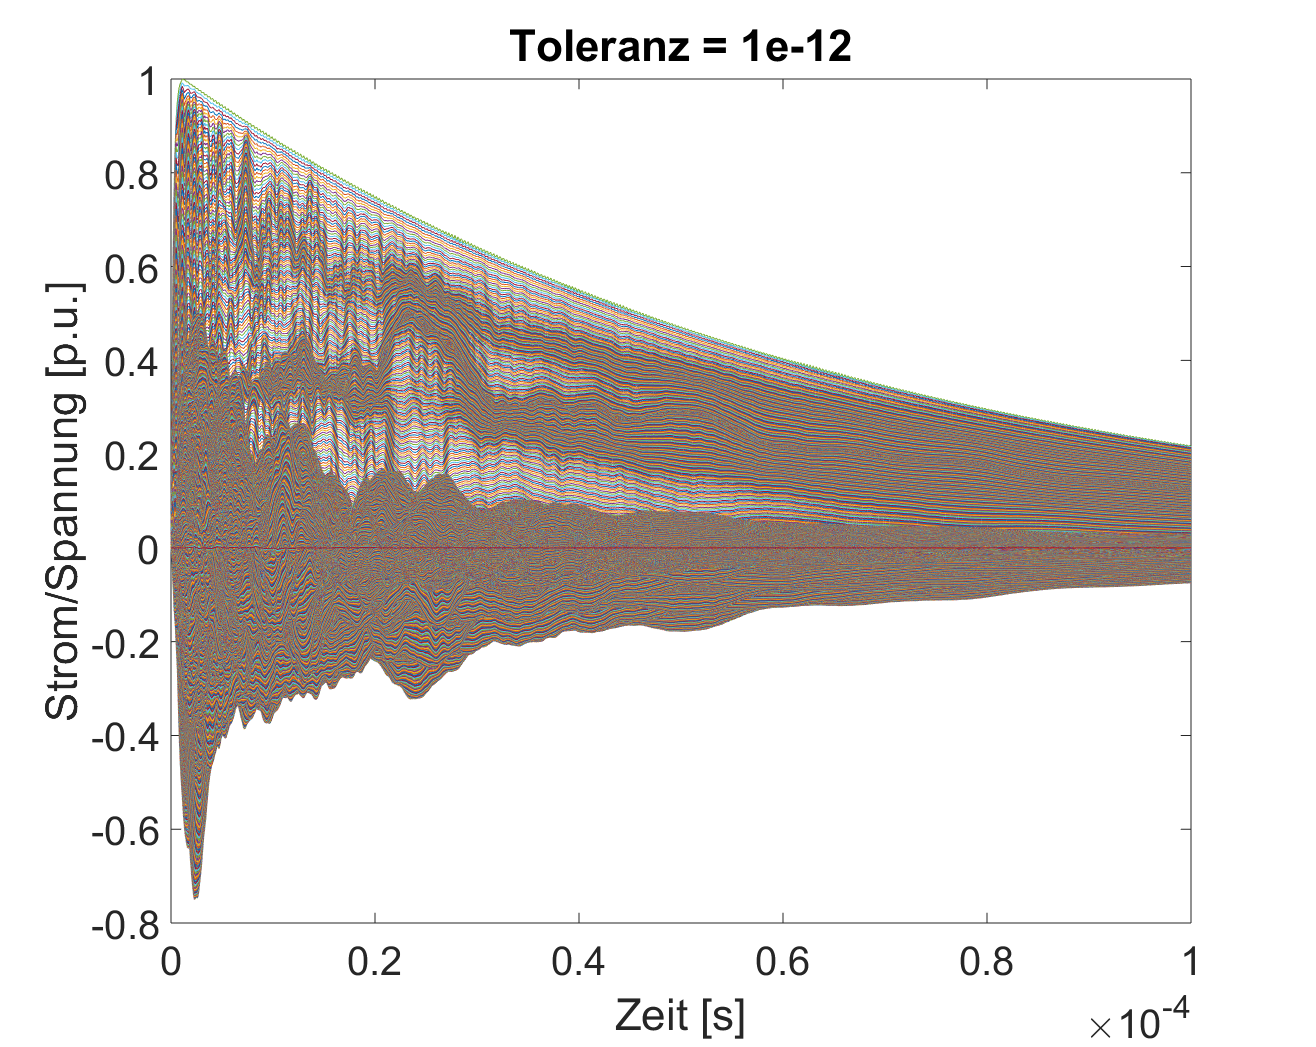
\includegraphics[width=\linewidth]{./trafo/images/svd12.png}
	    \end{minipage}
		\begin{minipage}{.5\textwidth}
	        \centering
	        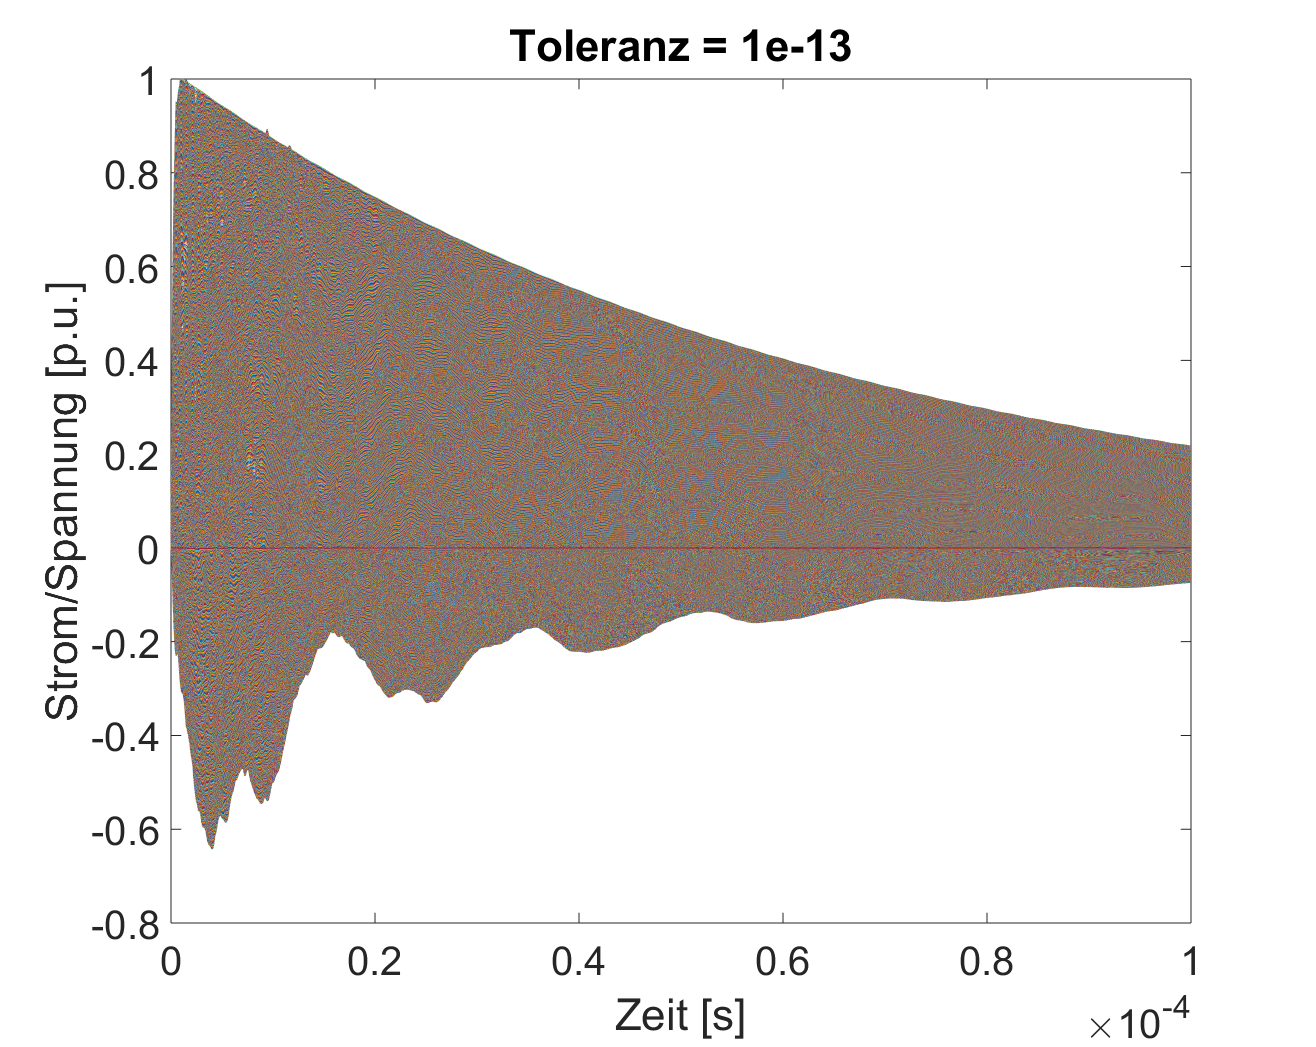
\includegraphics[width=\linewidth]{./trafo/images/svd13.png}
	    \end{minipage}%
	    \begin{minipage}{.5\textwidth}
	        \centering
	        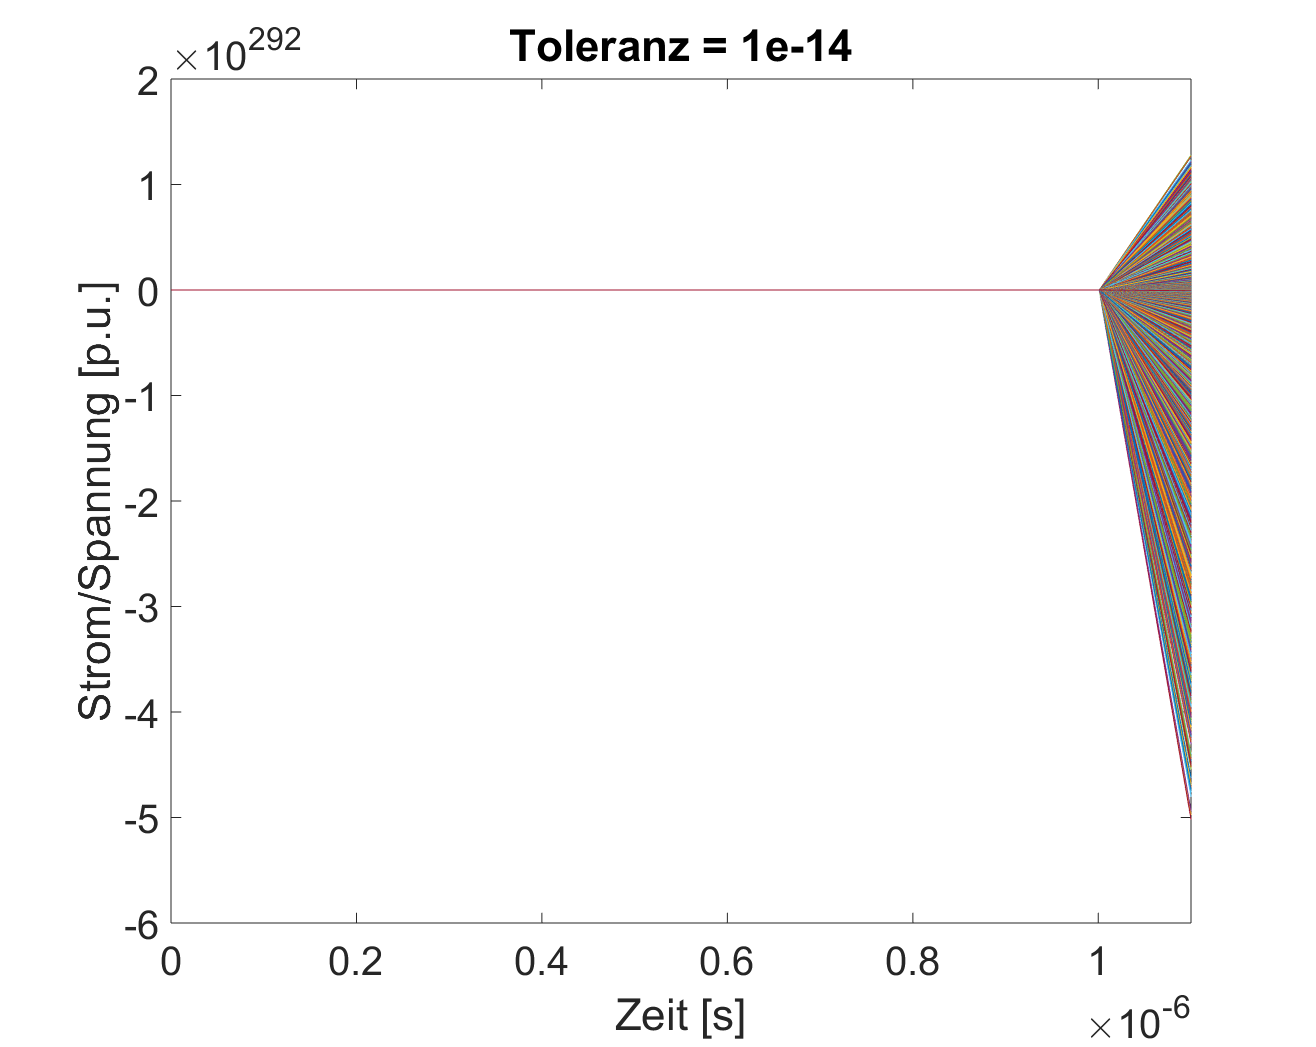
\includegraphics[width=\linewidth]{./trafo/images/svd14.png}
	    \end{minipage}
	    \caption{Numerische Berechnungen mit verschiedenen Toleranzen. Abgebildet sind Str"ome und Spannungen s"amtlicher Windungen. In der Abbildung unten rechts ist ersichtlich, dass die L"osungen bei einer zu klein gew"ahlten Toleranz explodieren und die L"osungen divergieren (es sei auf die Skala der $y$-Achse hingewiesen). }
	    \label{trafo:SVDTol}
	\end{figure}

\subsection{Exaktes L"osungsverfahren}
Eine stabile L"osung konnte mit dem \texttt{ode45}-L"osungsverfahren von Matlab bereits gefunden werden, allerdings ist der ben"otigte Zeitaufwand viel zu hoch. Aus diesem Grunde stellt sich die Frage, ob das Gleichungssystem \ref{trafo:symmetricalDGL} nicht auch exakt gel"ost werden kann.

Als Motivation wird eine gew"ohnliche Differentialgleichung erster Ordnung in einer Dimension betrachtet. 
\begin{equation*}
	\dot{x}(t) = a x(t) + b(t)
	\label{trafo:1D_DGL}
\end{equation*}
Diese Differentialgleichung l"asst nach
\begin{equation*}
	x_h(t) = x_0 e^{\lambda t}
	\label{trafo:homogene_Loesung}
\end{equation*}
aufl"osen, wobei $x_h$ die homogene L"osung ist. Den Fehlerterm wird im n"achsten Abschnitt etwas genauer betrachtet. 

Es gilt nun, die Matrix $A$ zu diagonalisieren und somit zu entkoppeln. Pr"adestiniert daf"ur w"are wiederum die Singul"arwertzerlegung. In der Anwendung zeigte sich leider, dass die Resultate aufgrund der unsymmetrischen Matrix $A$ nicht mit dem Erwarteten "ubereinstimmen und deshalb muss einen anderen Weg gefunden werden. Eine weitere M"oglichkeit ist die Eigenwertzerlegung. Wird die Eingangsinduktivit"at $L_\mathrm{in}$ in der Gleichung \ref{trafo:symmetricalDGL} nicht allzu klein gew"ahlt, l"asst sich das System tats"achlich l"osen.

Die Eigenwertzerlegung lautet $A = V\Lambda V^{-1}$ und angewendet auf das Differentialgleichungssystem 
\begin{align*}
	\dot{x} &= Ax + B \\
	\dot{x} &= V \Lambda \underbrace{V^{-1} x}_{y} + B \\
	\underbrace{V^{-1} \dot{x}}_{\dot{y}} &= \underbrace{V^{-1}V}_{E} \Lambda y + V^{-1} B \\
	\dot{y} &= \Lambda y + V^{-1} B
\end{align*}
wird die L"osung zu
\begin{equation}
	y(t) = y_0 e^{\Lambda t} + F(t)
	\label{trafo:TransfDGL}
\end{equation}
mit $y_0 = V^{-1}x_0$ und $F(t)$ als Fehlerterm.

Das Differentialgleichungssystem l"asst sich nun exakt\footnote{'exakt' bedeutet nicht, dass es keine numerische Fehler besitzt, denn diese wird es gewiss geben. Mit 'exakt' ist die soeben pr"asentierte L"osungsmethode gemeint. Der Gegensatz dazu ist ein numerisches L"osungsverfahren, welches das Gleichungssystem mittels Solvern f"ur gew"ohnliche Differentialgleichungen versucht zu l"osen.} l"osen. Es gilt nun, den Fehlerterm $B$ in die L"osung einzubinden, denn nur durch diesen Fehlerterm, dass heisst in diesem Falle den Blitzstoss, wird die Anwendung erst interessant.

Der Unterschied der Rechengeschwindigkeit zwischen der numerischen und exakten L"osung ist in Abbildung \ref{trafo:ode45vsExact} dargestellt. Der Fehlerterm f"ur die exakte L"osung wird diejenige Implementation verwendet, welche im n"achsten Abschnitt genauer behandelt wird. 

	\begin{figure}
		\centering
		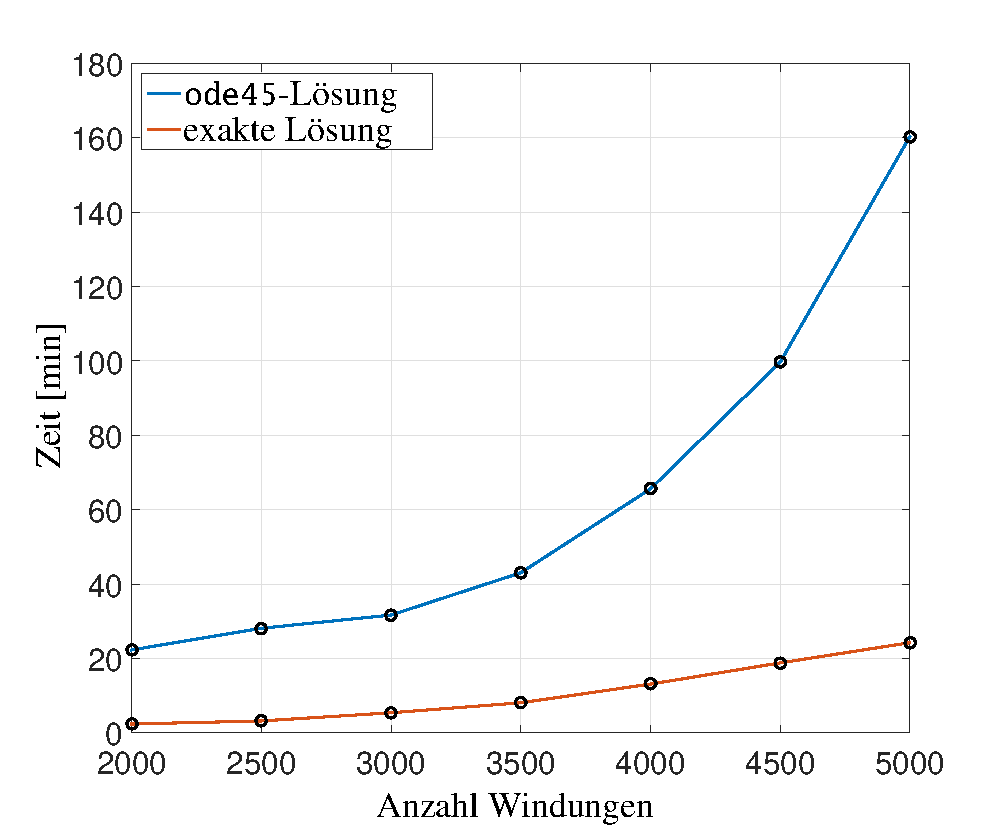
\includegraphics[width=0.6\textwidth]{./trafo/images/ode45vsExact.pdf}
		\caption{Unterschied zwischen dem \texttt{ode45}-L"osungsverfahren von Matlab und dem exakten L"osungsverfahren, welches im Abschnitt \ref{trafo:SecOptimierung} pr"asentiert wird.}
		\label{trafo:ode45vsExact}
	\end{figure}


\subsection{Fehlerterm und Schrittweite}
Da es sich beim Fehlerterm nicht nur um eine Funktion, sondern auch um ein gemessenes Signal handelt, welches somit quantisiert ist, muss der Fehlerterm "uber einen gewissen Zeitschritt betrachtet werden.

\subsubsection{Konstanter St"orterm}
Ein m"oglicher Ansatz ist es, denn Fehlerterm f"ur die Schrittweite $h$ als konstant zu betrachten. Die Gleichung \ref{trafo:TransfDGL} kann nun als
\begin{equation*}
	Y_i = Y_{i-1} e^{\Lambda h}  + h B_{i-1}
\end{equation*}
geschrieben werden. $Y_i$ und $B_i$ sind jeweils Vektoren der L"osungsmatrix respektive Fehlertermmatrix. 

\subsubsection{Linear Interpolierter St"orterm}
Es liegt nat"urlich nahe den St"orterm etwas sinnvoller zu implementieren. Denn eine Treppenfunktion, wie sie soeben beschrieben wurde, verh"alt sich bei grossen Schrittweiten $h$ sehr schlecht. Ein besseres Verhalten kann eine lineare Interpolation
\begin{equation*}
	b(t) = b_0 + \frac{b_1 - b_0}{h}t
\end{equation*}
besitzen. Der beliebige St"orterm $b(t)$ wird im Intervall $[0,h]$ durch diese lineare Interpolation zwischen den Werten $b_0 = b(0)$ und $b_1 = b(h)$ approximiert \cite{trafo:Mueller}.

Die homogene L"osung der Gleichung ist bereits bekannt (\ref{trafo:homogene_Loesung}), die partikul"are muss mit Hilfe der Variation der Konstante gefunden werden. Der Ansatz
\begin{equation*}
	y_p(t) = C(t)e^{\lambda t}
\end{equation*}
wird in die homogene Gleichung eingesetzt \cite{trafo:Mueller}.
\begin{align*}
	\dot{y}_p(t) &= \lambda y_p(t) + b(t) \\
	\dot{C}(t)e^{\lambda t} + C(t)\lambda e^{\lambda t} &= C(t) \lambda e^{\lambda t} + b(t) \\
	\dot{C}(t) &= e^{-\lambda t} b(t) \\
	C(t) &= \int_{0}^{t} e^{\lambda \xi} b(\xi) d\xi = \int_{0}^{x} e^{\lambda \xi} \left(b_0 + \xi \frac{b_1 - b_0}{h}\right) d\xi
\end{align*}
Da am Schluss der Fall $x = h$ anliegt und somit $y_1 = y(h)$ berechnet werden muss, braucht die allgemeine Form von $C(t)$ nicht ausgerechnet zu werden. Die Berechnung mit Maxima ergibt \cite{trafo:Mueller}
\begin{equation}
	y_1 = y_0 e^{\lambda h} + \frac{b_0 e^{\lambda h} - b_1}{\lambda} + \left(b_1 - b_0\right) \frac{e^{\lambda h} -1}{h \lambda^2}
	\label{trafo:linInterp}
\end{equation}
oder f"ur das Differentialgleichungssystem
\begin{equation}
	Y_1 = Y_0 e^{\Lambda h} + \frac{B_0 e^{\Lambda h} - B_1}{\Lambda} + \left(B_1 - B_0\right) \frac{e^{\Lambda h} -1}{h \Lambda^2}.
	\label{trafo:exakteLoesung}
\end{equation}

\subsubsection{Vergleich}
In Abbildung \ref{trafo:interpVergleich} werden konstante Fehlerterme (oben) und linear interpolierte Fehlerterme (unten) mit verschiedener Anzahl Zeitschritte dargestellt. Es ist sehr gut ersichtlich, dass die lineare Interpolation des Fehlerterm mit relativ wenigen Zeitschritten an das gew"unschte Ziel kommt, wohingegen der konstantgehaltene Fehlerterm wesentlich mehr Zeitschritte f"ur die selbe Genauigkeit ben"otigt. 

Abbildung \ref{trafo:differenceTimestep} zeigt der Unterschied der Berechnungszeiten des konstanten und des linear interpolierten St"orterm. Beide dauern ungef"ahr gleich lange und wachsen linear mit der Anzahl Zeitschritte. Der wesentliche Unterschied besteht darin, dass die lineare Interpolation bei sehr viel wenigeren Zeitschritten bereits eine akzeptable L"osung ergibt (gr"une Kreuze).
	\begin{figure}
	    \centering
	    \begin{minipage}{.32\textwidth}
	        \centering
	        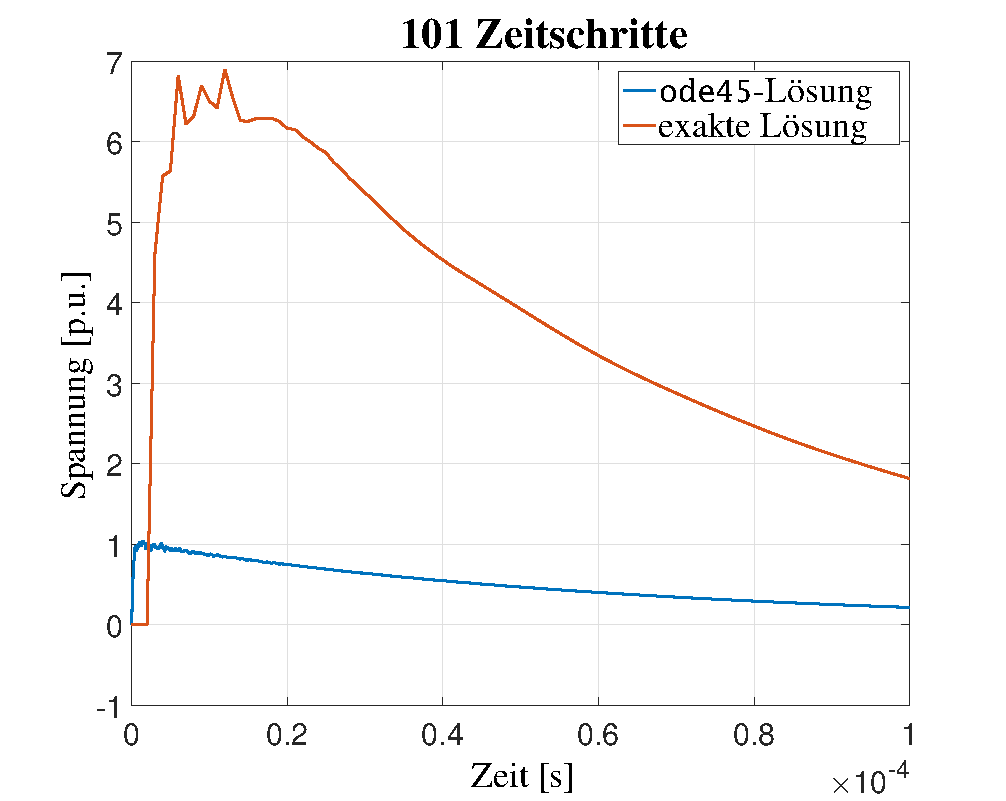
\includegraphics[width=\linewidth]{./trafo/images/Sprung101.pdf}
	    \end{minipage}%
	    \begin{minipage}{.32\textwidth}
	        \centering
	        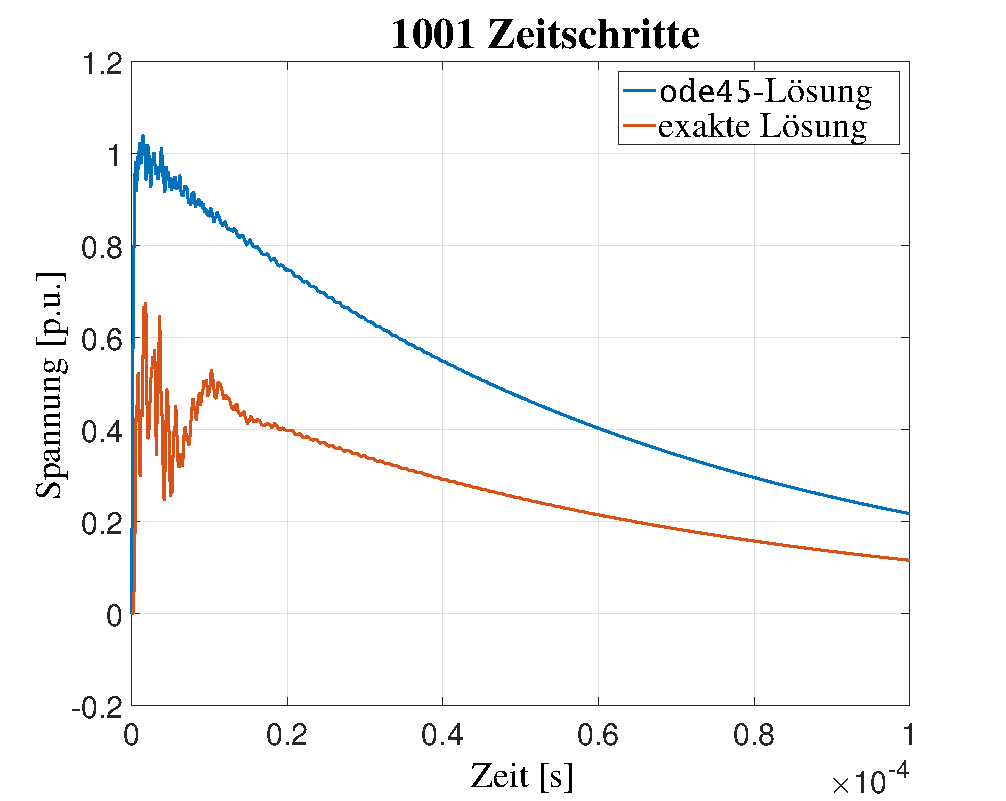
\includegraphics[width=\linewidth]{./trafo/images/Sprung1001.pdf}
	    \end{minipage}
	    \begin{minipage}{.32\textwidth}
	        \centering
	        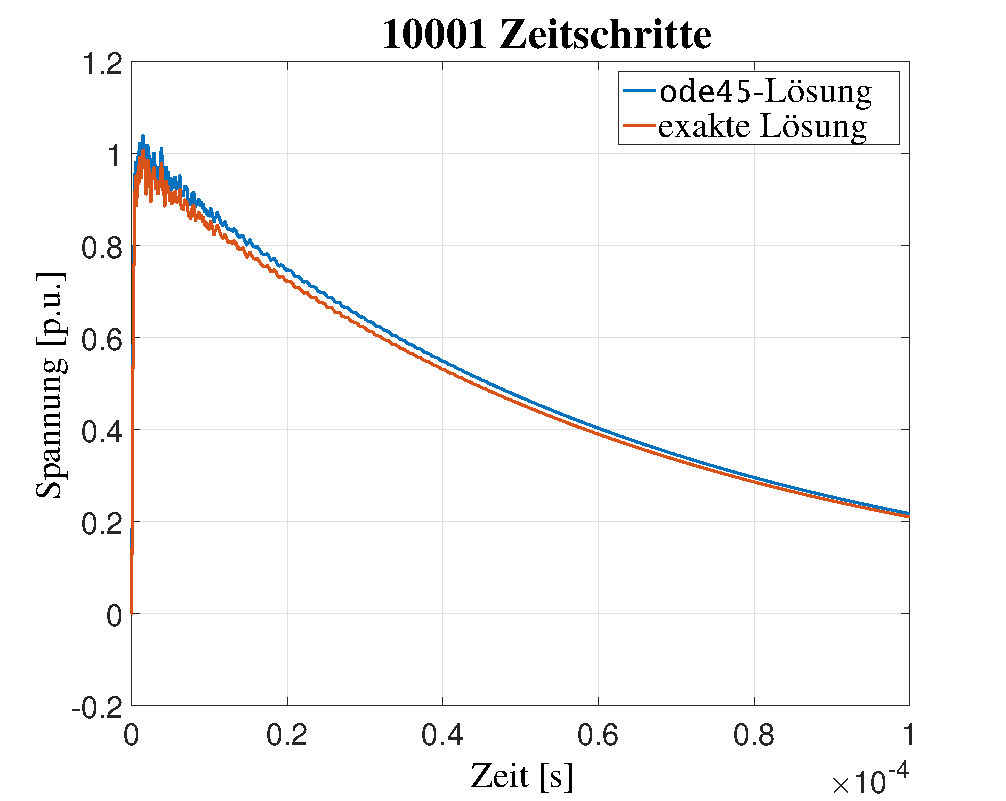
\includegraphics[width=\linewidth]{./trafo/images/Sprung10001.pdf}
	    \end{minipage}
		\begin{minipage}{.32\textwidth}
	        \centering
	        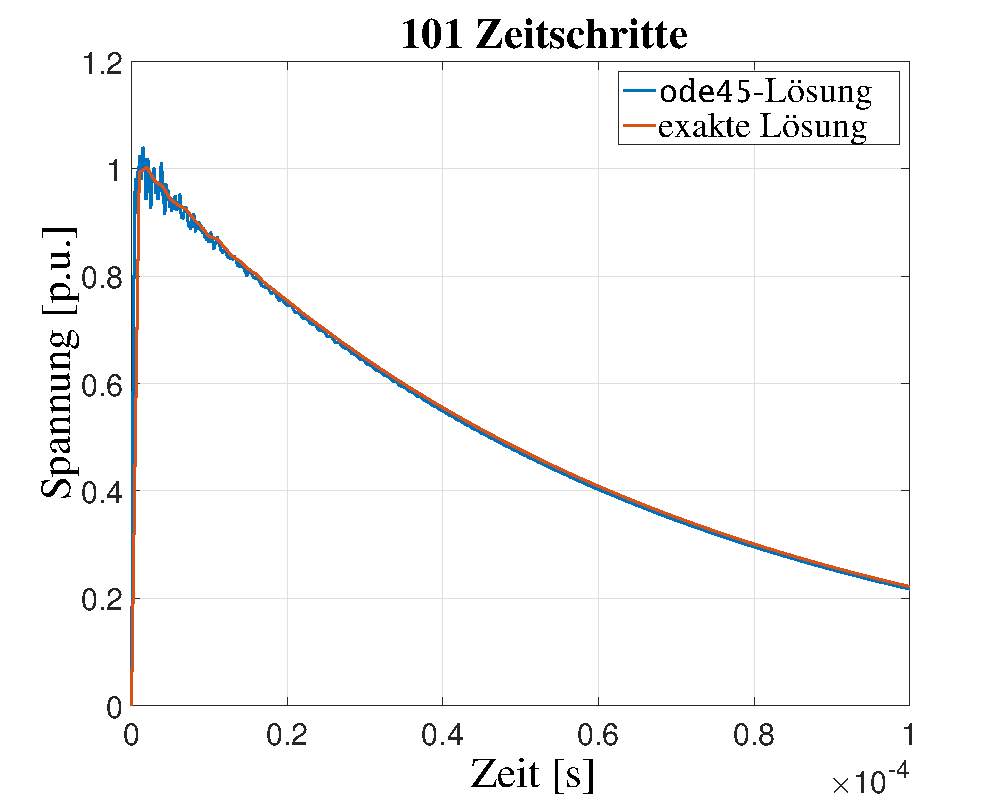
\includegraphics[width=\linewidth]{./trafo/images/Interp101.pdf}
	    \end{minipage}%
	    \begin{minipage}{.32\textwidth}
	        \centering
	        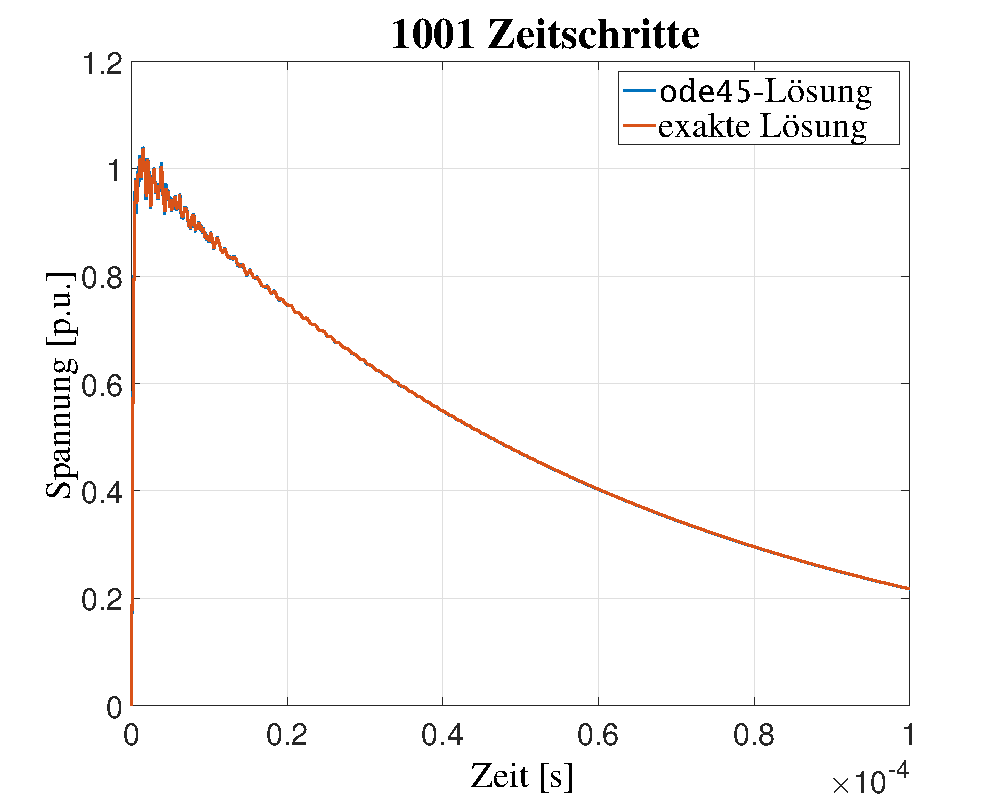
\includegraphics[width=\linewidth]{./trafo/images/Interp1001.pdf}
	    \end{minipage}
	    \begin{minipage}{.32\textwidth}
	        \centering
	        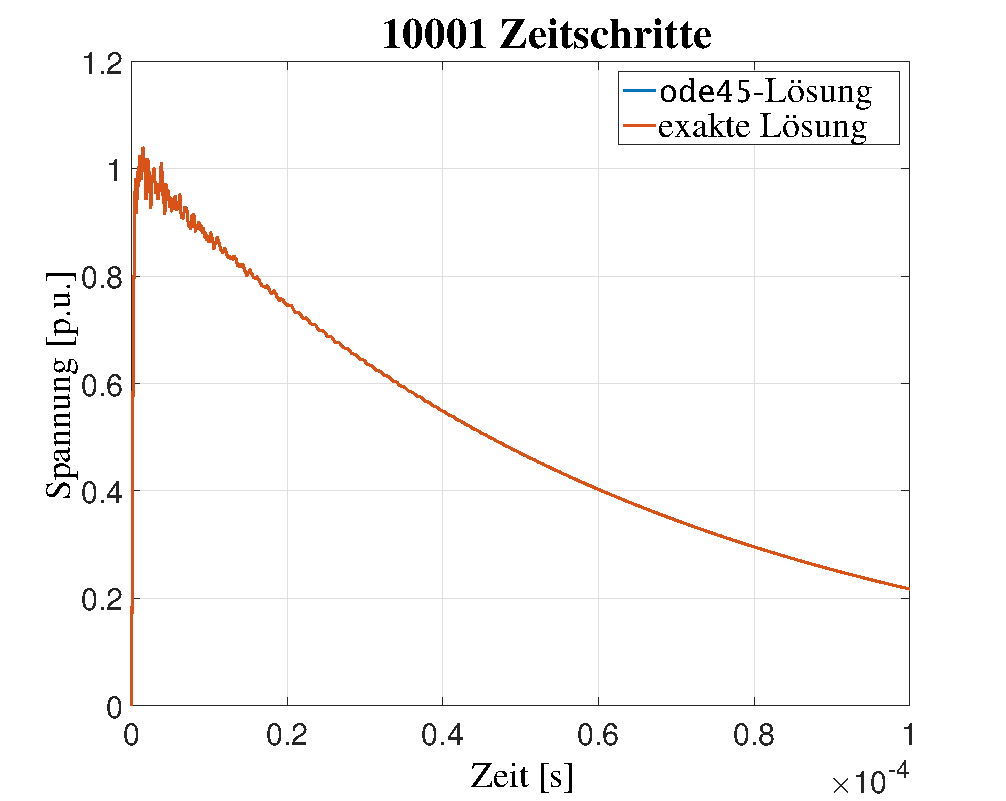
\includegraphics[width=\linewidth]{./trafo/images/Interp10001.pdf}
	    \end{minipage}
	    \caption{Unterschied konstanter (oben) und linearer interpolierter (unten) St"orterm mit verschiedenen Anzahl Zeitschritten.}
	    \label{trafo:interpVergleich}
	\end{figure}

	
	\begin{figure}
			\centering
			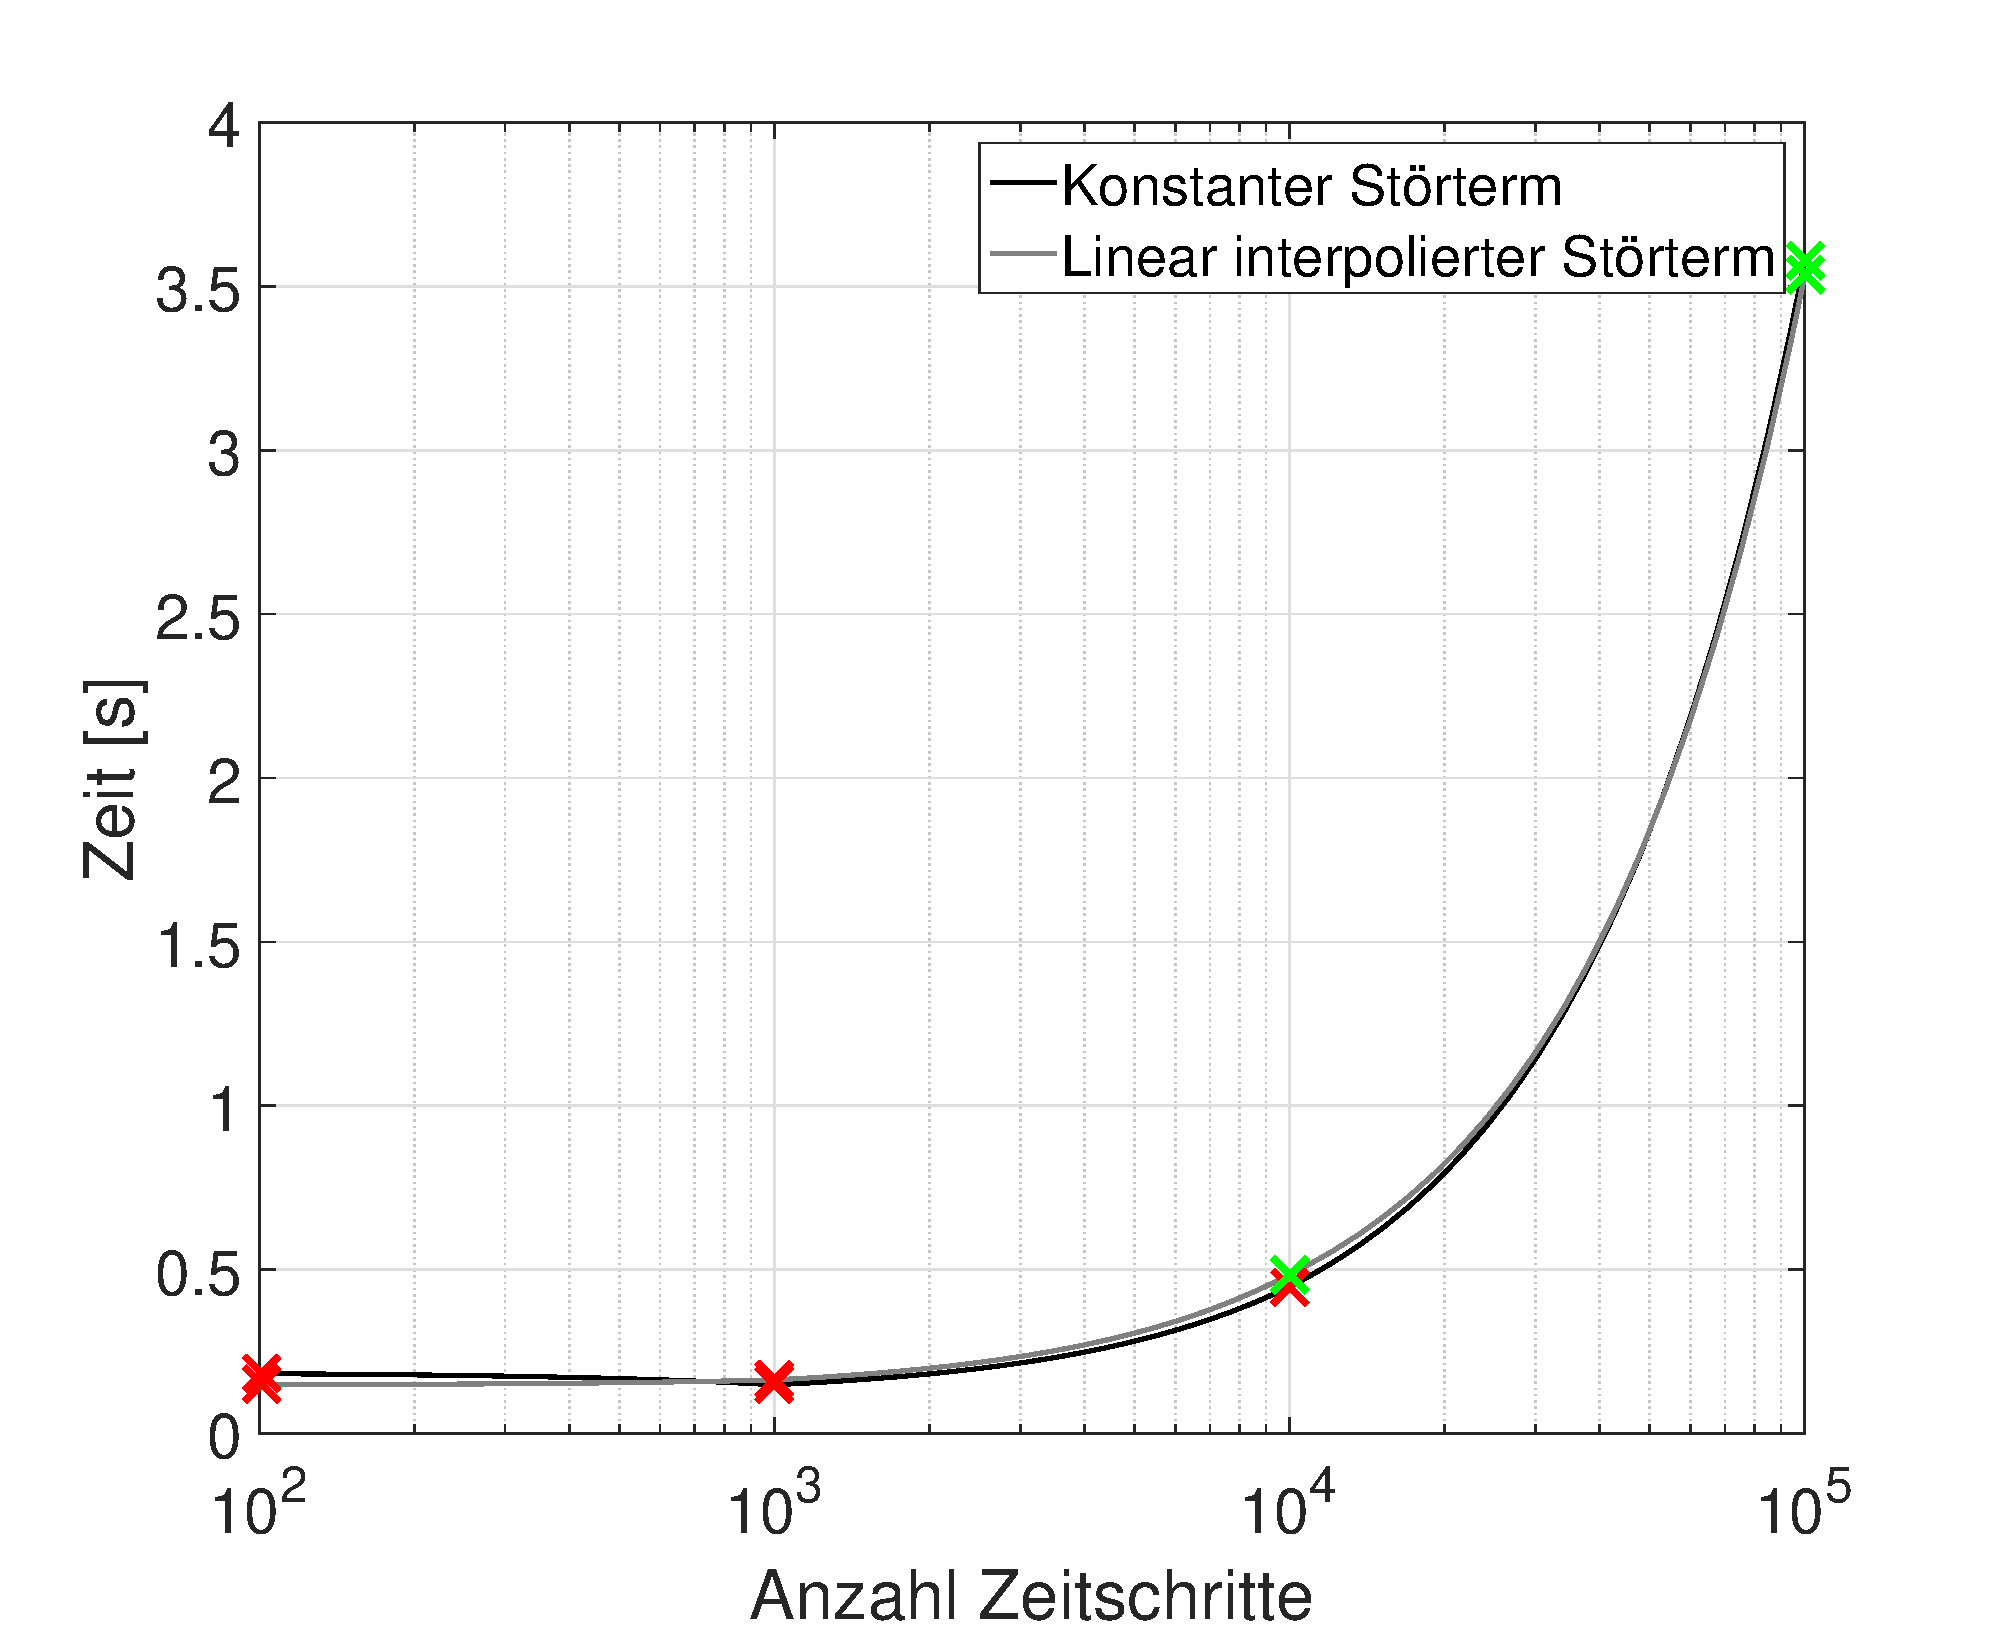
\includegraphics[width=0.9\textwidth]{./trafo/images/differenceTimestep.pdf}
			\caption{Unterschied konstanter und linearer interpolierter St"orterm in Abh"angigkeit der Zeitschritte. Akzeptable L"osungen sind mit einem gr"unen Kreuz markiert, L"osungen welche verworfen werden m"ussen, mit einem roten Kreuz.}
			\label{trafo:differenceTimestep}
	\end{figure}
		
\subsection{Optimierungen \label{trafo:SecOptimierung}}

Ein wichtiger Punkt bei L"osungsverfahren ist die Optimierung. Einen grossen Optimierungsschritt ist bereits beim "Ubergang von der \texttt{ode45}- zur exakten L"osung passiert. Potential zur Verbesserung ist jedoch immer vorhanden.

Der wesentliche Teil der Berechnung, welche beeinflusst werden kann, ist die \textit{for}-Schleife. Diese wird so oft durchlaufen, wie die Anzahl der Schritte gew"ahlt wurde. Deshalb soll das Ziel sein, m"oglichst wenig in dieser Schleife zu berechnen. 

\subsubsection{Exponentialfunktion der Eigenwerte}
Die Gleichung \ref{trafo:exakteLoesung} besitzt eine Konstante $e^{\Lambda h}$, welche bei jedem Zeitschritt mit den neuen Anfangswerten multipliziert wird. Es macht also Sinn, diese Konstante einmal vor der Schleife zu berechnen und als Variable abzuspeichern. Da es sich bei der Matrix $\Lambda$ um eine Diagonalmatrix handelt, h"alt sich auch der Speicherbedarf der Konstante in Grenzen (es sind dies $2n + 1$ Variablen in einer \textit{sparse}-Matrix). 

\subsubsection{Lineare Interpolation}
Die soeben vorgestellte lineare Interpolation \ref{trafo:linInterp} kann mittels Umformungen in die Darstellung 

\begin{equation*}
	y_1 = y_0 \cdot e^{\lambda h} + b_0 \underbrace{\left(\left(\frac{e^{\lambda h}}{\lambda} - \frac{e^{\lambda h}}{h\lambda ^2}\right) + \frac{1}{h \lambda^2}\right)}_{a_0} + b_1 \underbrace{\left(\frac{e^{\lambda h}}{h \lambda^2} - \frac{1}{\lambda} - \frac{1}{h \lambda^2}\right)}_{a_1}
\end{equation*} 
gebracht werden. Die Konstanten $a_0$ und $a_1$ k"onnen wiederum vor der Schleife einmal berechnet werden. Die lineare Interpolation kann jetzt als 
\begin{equation*}
	y_1 = y_0 \cdot e^{\lambda h} + a_0 \cdot b_0 + a_1 \cdot b_1
\end{equation*}
geschrieben werden. 

Da sich bei diesem Problem nur die Eingangspannung "andert, ist die Ver"anderung vom transformiertem Vektor $b_0$ zu $b_1$ f"ur alle Elemente dieselbe Zahl $b$. Die Interpolation kann noch etwas einfacher als
\begin{equation*}
	y_1 = y_0 \cdot e^{\lambda h} + (a_0 + b \cdot  a_1) \cdot b_0
\end{equation*}
geschrieben werden, wenn $b$ die Differenz der zwei Vektoren $b_0$ und $b_1$ ist. 

\subsubsection{Implementation}
Der Matlab-Code kann jetzt folgendermassen geschrieben werden.

{\scriptsize \lstinputlisting{./trafo/code/compact.m}}


\subsubsection{Vergleich}

Um die Performance zu testen, wird eine sehr schlechte Implementation gew"ahlt, welche den Fehlerterm lineare interpoliert. Im Gegensatz zum soeben gezeigten Code werden in dieser schlechten Variante alle Konstante in der \textit{for}-Schleife berechnet. Jeder einzelner Zeitschritt dauert bei dieser Berechnung ca. \SI{130}{\milli\second}. 

Als Vergleich wird die schnellste Optimierung verwendet (Matlab-Code von oben). Die Berechnungszeit f"ur jeden einzelnen Zeitschritt konnte bis auf \SI{35}{\micro \second} reduziert werden. Die Grafik \ref{trafo:Optimierung} zeigt den Unterschied in einer doppelt logarithmischen Grafik. Die Optimierung hat auf ein hervorragend schnelles Verfahren gef"uhrt.

\begin{figure}
	\centering
	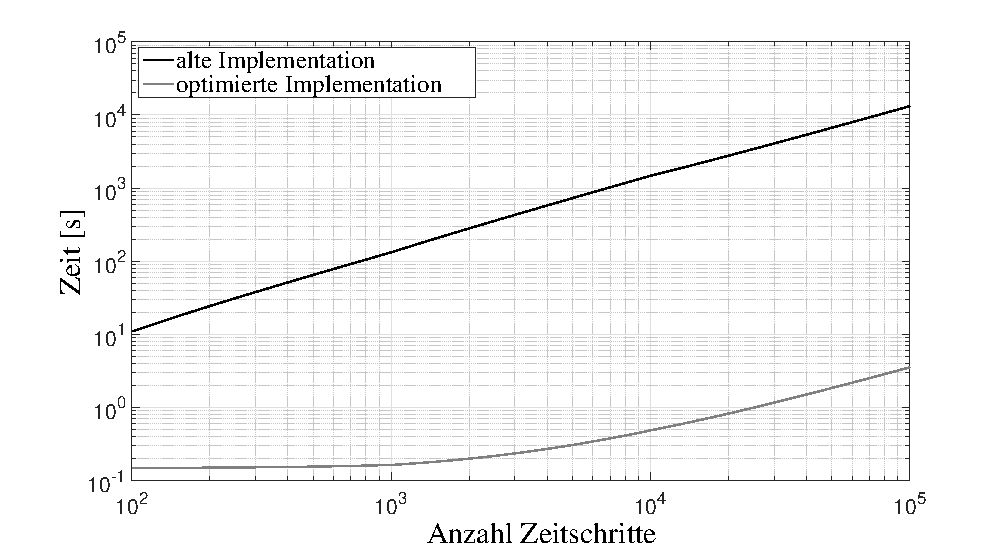
\includegraphics[width=0.9\textwidth]{./trafo/images/differenceOptimization.pdf}
	\caption{Unterschied zwischen einer sehr schlechten und einer guten Implementierung bei einem Trafomodell mit 500 Windungen.}
	\label{trafo:Optimierung}
\end{figure}

\section{Anwendung der gefundenen L"osungen}

\begin{figure}
	\centering
	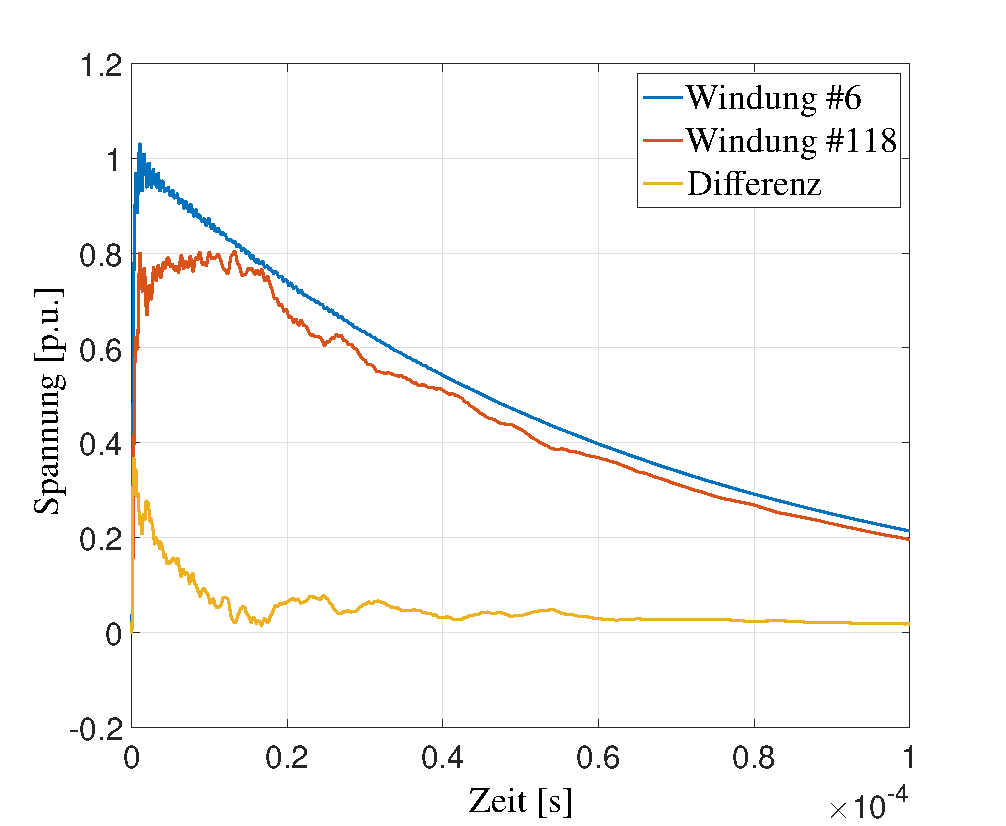
\includegraphics[width=0.7\textwidth]{./trafo/images/solution.pdf}
	\caption{Spannung zwischen Windung 6, 118 und deren Differenz.}
	\label{trafo:solution}
\end{figure}

Schlussendlich k"onnen die gefundenen L"osungen wieder in das CAD-Modell eingelesen werden, damit das elektrische Feld simuliert werden kann. Somit kann festgestellt werden, wo sich Schwachstellen im Transformator befinden und diese allenfalls verbessert werden.

Interessant ist nat"urlich immer der gr"osste Spannungsunterschied zwischen benachbarten Windungen. In diesem Beispiel ist dies zwischen dem Layer 1 und 2 zwischen Windung 6 und 118.

Diese L"osung wurde bereits in Abbildung \ref{trafo:solution} pr"asentiert. Das elektrische Feld zum Zeitpunkt der gr"ossten Spannungsdifferenz ist in den Abbildungen \ref{trafo:E-Field} und \ref{trafo:E-FieldZoom} dargestellt. 

\begin{figure}
	\centering
	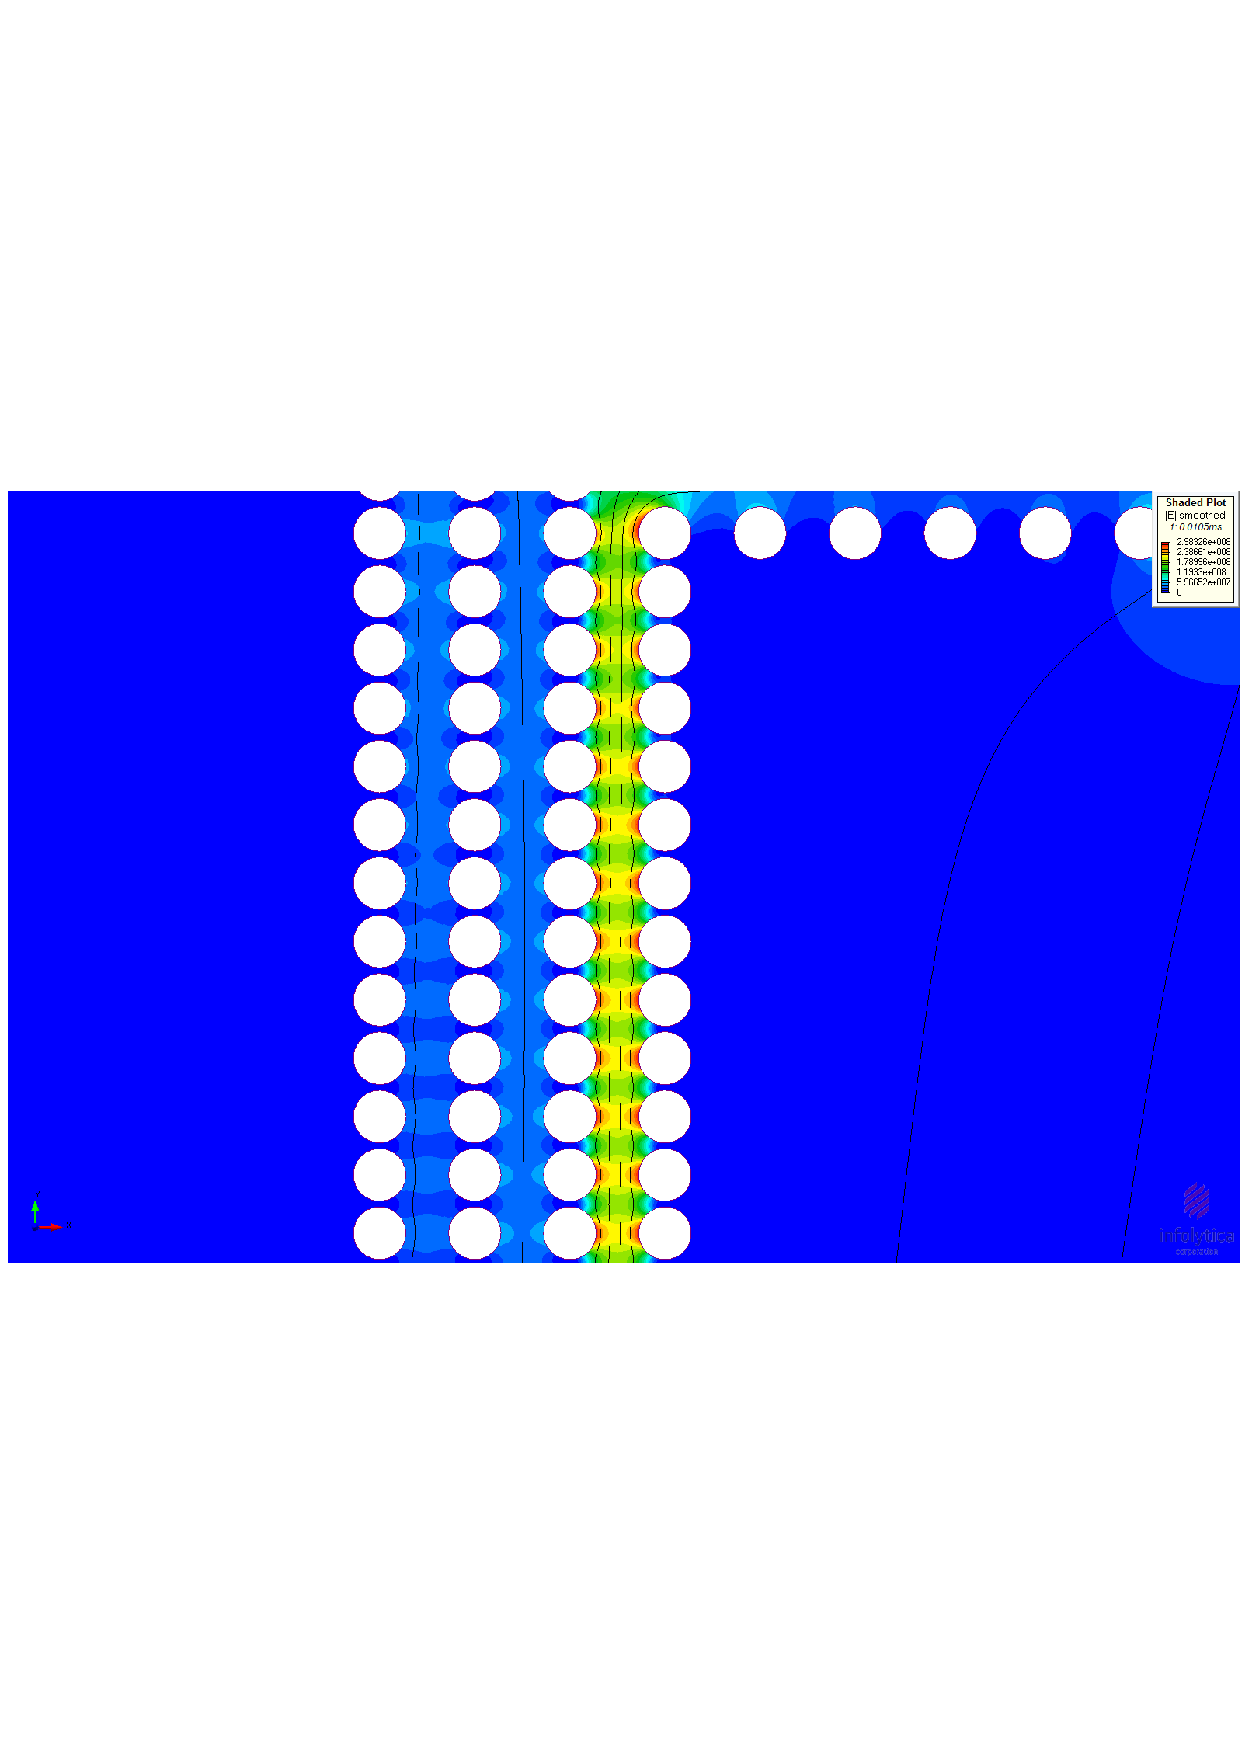
\includegraphics[width=\textwidth]{./trafo/images/BIL_VoltageTrans.pdf}
	\caption{Elektrisches Feld zwischen den ersten paar Layern.}
	\label{trafo:E-Field}
\end{figure}

\begin{figure}
	\centering
	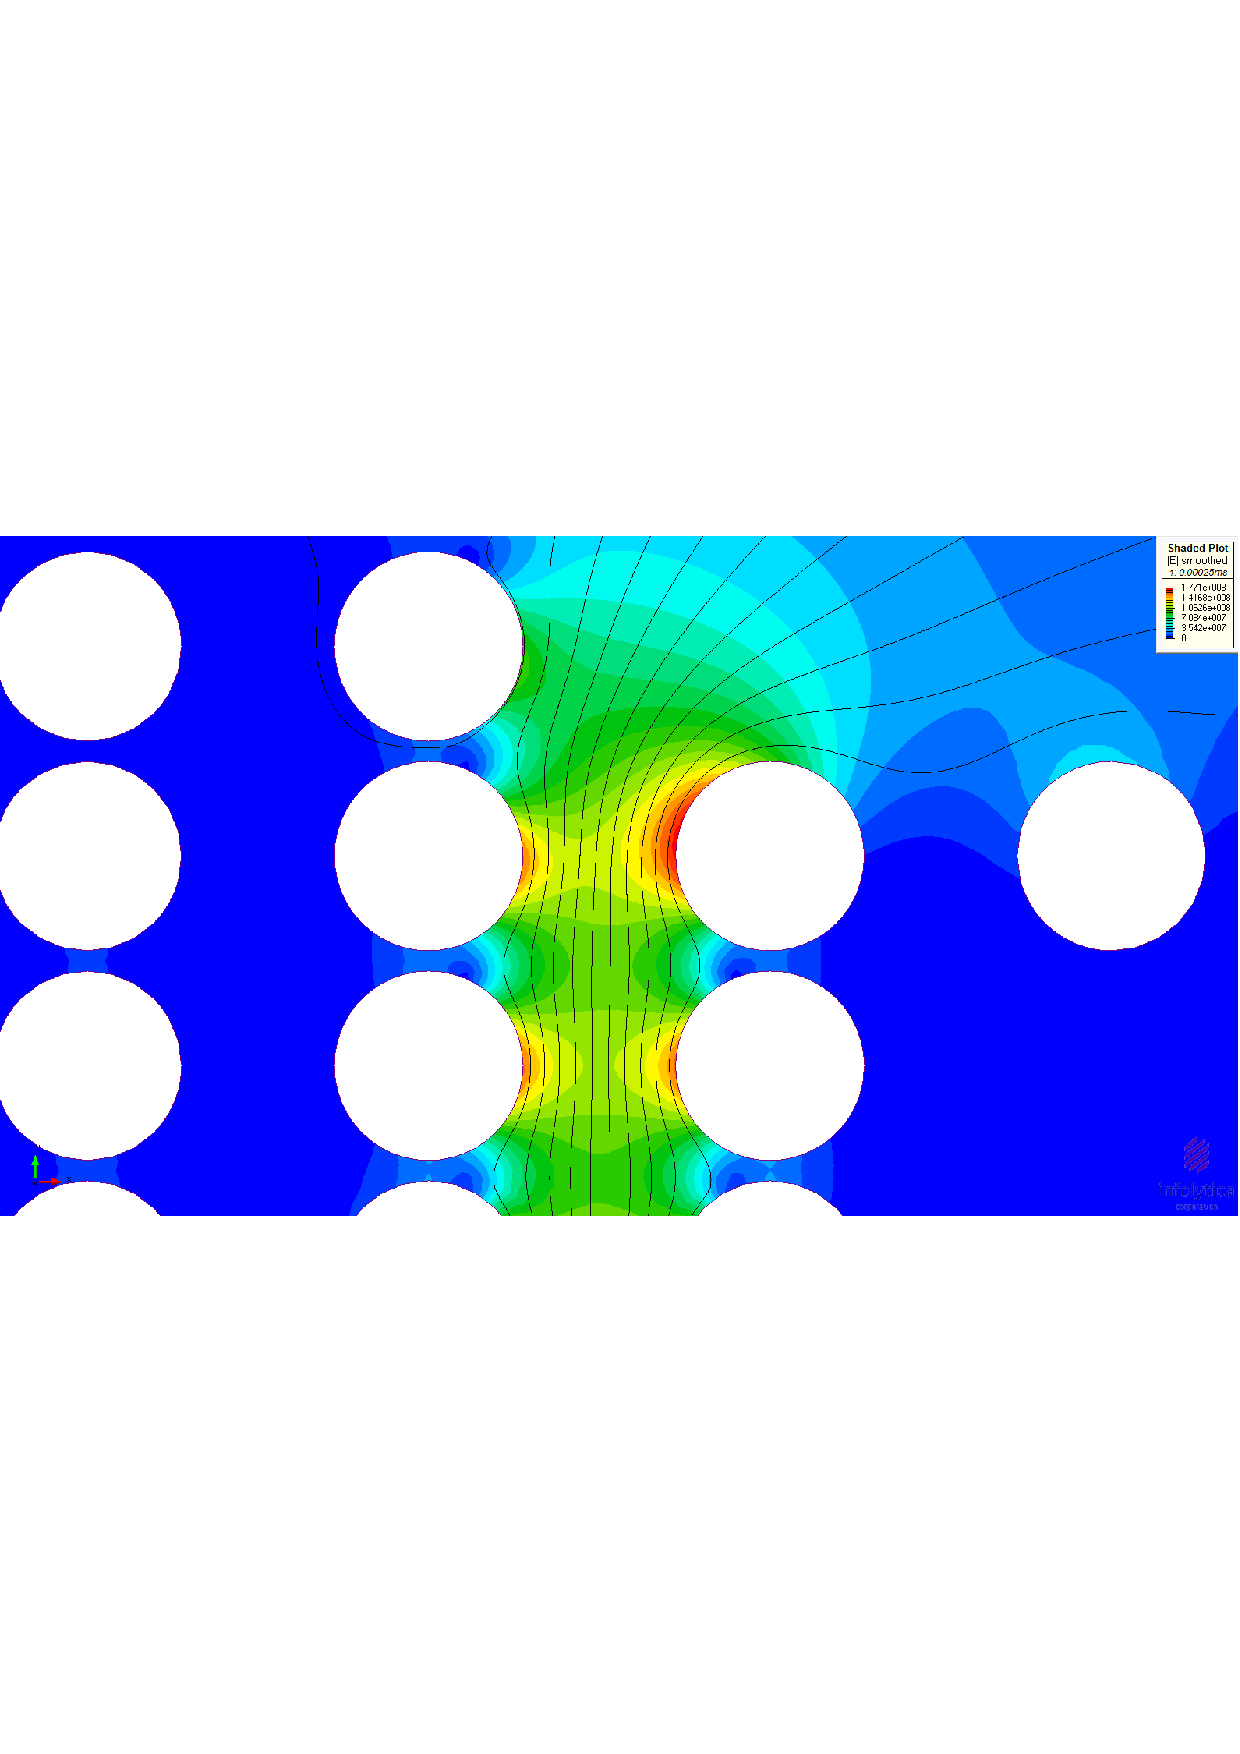
\includegraphics[width=\textwidth]{./trafo/images/VoltageTrans.pdf}
	\caption{Elektrisches Feld zwischen Windung 6 und 118.}
	\label{trafo:E-FieldZoom}
\end{figure}

Da die Herstellung von Transformatoren nie optimal abl"auft, k"onnen sich auch Luftblasen im Epoxidharz bilden. Diese Luftblasen, auch Lunker genannt, verst"arken das elektrische Feld zus"atzlich und schw"achen somit den Transformator im Fehlerfall. Ein m"ogliches Szenario ist in Abbildung \ref{trafo:E-FieldBubble} pr"asentiert. 

\begin{figure}
	\centering
	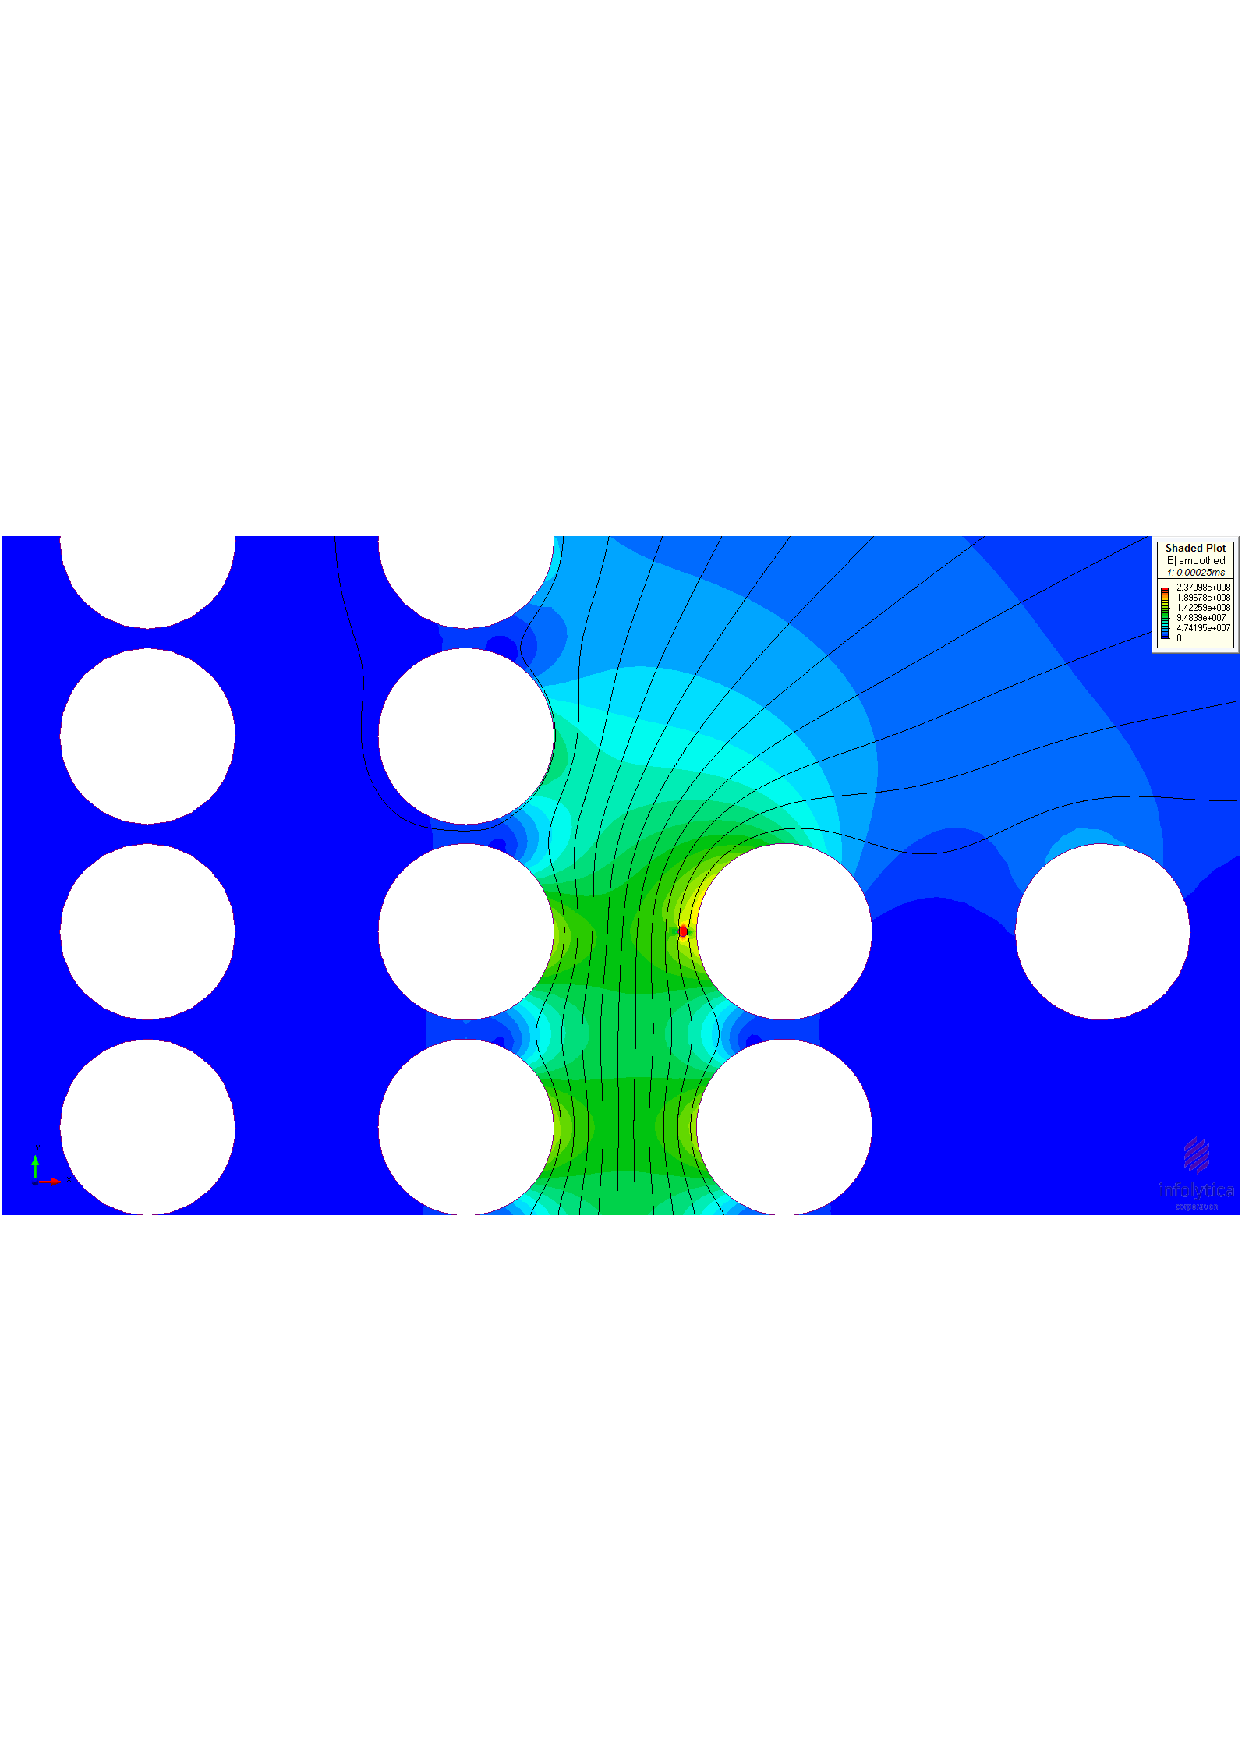
\includegraphics[width=\textwidth]{./trafo/images/VoltageTrans_bubble_turn6_10u_9u.pdf}
	\caption{Elektrisches Feld zwischen Windung 6 und 118 mit simulierter Luftblase (Lunker).}
	\label{trafo:E-FieldBubble}
\end{figure}

\subsection{Schlussfolgerung}
Das Problem konnte erfolgreich formuliert werden und es l"asst sich in der Praxis auch erfolgreich l"osen. Mit mathematischen Hilfsmitteln ist es nun m"oglich, die Spannungsverteilung in Transformatoren mit einer grosser Anzahl Windungen zu berechnen. Teilweise muss die Eingangsinduktivit"at etwas angepasst werden, wenn die Anzahl Windungen sehr gross ist. Da aber bei einer hoher Anzahl Windungen die Induktivit"at des Transformators sowieso sehr gross ist, wirkt sich eine gr"ossere Eingangsinduktivit"at nicht wesentlich auf das Resultat aus.

Es konnte gezeigt werden, dass sich das Problem numerisch und analytisch l"osen l"asst und vor allem in der Rechengeschwindigkeit enorme Unterschiede bestehen. Ebenfalls l"asst sich der Blitzimpuls linear interpolieren, welches wesentlich schneller zu einer vern"unftigen L"osung f"uhrt.

Der L"osungsansatz wurde in Matlab soweit optimiert, wie es m"oglich ist. Will die Rechengeschwindigkeit noch erh"oht werden, muss eine eigene Implementation in \texttt{C} und/oder eine Parallelisierung der Berechnung erfolgen.

\printbibliography[heading=subbibliography]
\end{refsection}
